\documentclass[10pt,twocolumn]{article}

% ------------------------------------------------------------------------------
% Packages for Professional Typography and Layout
% ------------------------------------------------------------------------------
\usepackage[utf8]{inputenc}
\usepackage[T1]{fontenc}
\usepackage{lmodern}
\usepackage[margin=0.75in,columnsep=0.25in]{geometry}
\usepackage{amsmath,amssymb,amsfonts}
\usepackage{booktabs}
\usepackage{graphicx}
\usepackage{subcaption}
\usepackage{algorithm}
\usepackage{algorithmic}
\usepackage{cite}
\usepackage{xcolor}
\usepackage{microtype}
\usepackage{url}
\usepackage[colorlinks=true,linkcolor=blue,citecolor=blue,urlcolor=blue]{hyperref}

% ------------------------------------------------------------------------------
% Custom Definitions and Formatting
% ------------------------------------------------------------------------------
\newcommand{\systemname}{\textsc{HACER-RAG}}

\newenvironment{IEEEkeywords}
  {\vspace{0.5em}\noindent\textbf{\textit{Keywords---}}\ignorespaces}
  {\vspace{1.0em}}

% Title and Authors
\title{\Large\textbf{\systemname: Evidence-Version-Aware KV-Cache Reuse and Selective Repair for On-Device Retrieval-Augmented Generation}}

\author{
  \textbf{Mobile Systems and Language Model Research Group}\\
  PortingLLM Research Project\\
  \texttt{\{systems-research, mobile-llm\}@portingllm.org}
}

\date{\today}

% ------------------------------------------------------------------------------
% Main Document Content
% ------------------------------------------------------------------------------
\begin{document}

\maketitle

% Section 1: Abstract & Keywords
\begin{abstract}
On-device Retrieval-Augmented Generation (RAG) enables privacy-preserving, low-latency question answering on resource-constrained mobile hardware. However, executing autoregressive Small Language Models (SLMs) on mobile CPUs incurs severe prompt-prefill latency when repeatedly encoding retrieved context. While precomputing and restoring Key-Value (KV) cache prefixes can eliminate redundant prefill computation, existing mobile runtimes treat KV-cache files as opaque conversational histories. This introduces a critical systems failure mode: \emph{silent stale-cache hallucination}, where outdated or revoked retrieved evidence preserved in serialized KV caches causes the model to generate factually incorrect responses without detection. Furthermore, dynamic context-capacity constraints and continuation-token boundary effects frequently trigger out-of-memory (OOM) aborts or silent truncation on memory-limited handsets.

In this paper, we present \textbf{HACER-RAG} (\textbf{H}ierarchical \textbf{A}daptive \textbf{C}ache, \textbf{E}vidence-version-aware \textbf{R}epair for on-device RAG), a mobile inference system designed for reliable and efficient local RAG on commodity Android smartphones. HACER-RAG pairs a canonical evidence layout with cryptographic chunk-level hashing to bind every KV cache segment to an explicit evidence version. When retrieved context changes, HACER-RAG executes a selective repair policy that preserves valid prefix KV tensors while triggering online prefill only for updated downstream chunks, falling back safely to clean scratch prefill under cache corruption. In addition, HACER-RAG introduces a JNI-level context-budget safety guard that dynamically enforces headroom constraints and models continuation boundary-token alignment. 

We evaluate HACER-RAG on a physical Xiaomi Redmi 12 5G smartphone (Qualcomm Snapdragon 4 Gen 2 SoC, Android 14) using a 4-bit quantized Gemma 2 2B model executing via \texttt{llama.rn} and \texttt{llama.cpp}. In a rigorous 90-matched-pair empirical scaling study across nine configurations ($K \in \{1, 2, 4\}$ chunks, $n_{\text{ctx}} \in \{512, 1024, 2048\}$), HACER-RAG achieves mean prompt-prefill compute reductions of \textbf{19.3--21.2\%} for $K=1$ (84 cached tokens), \textbf{38.5--40.4\%} for $K=2$ (158 cached tokens), and \textbf{86.1--86.7\%} for $K=4$ (341 cached tokens), delivering up to \textbf{3.65$\times$} end-to-end wall-clock speedup with zero native truncation and 100\% deterministic output parity. A balanced Two-Way ANOVA demonstrates that prefill reductions are strictly governed by cached token count ($F = 1920.56, p < 10^{-68}, \eta_p^2 = 0.979$), with no statistically significant main effect from context capacity ($p = 0.981$) or interaction ($p = 0.729$). In repeated multi-chunk RAG trials (9 matched pairs), HACER-RAG achieves a mean prefill reduction of \textbf{44.13\%} and a wall speedup of \textbf{1.63$\times$} while preserving 100\% multi-hop factual accuracy, incurring an average flash cache-load overhead of only 256.0~ms compared to 16.8~seconds of CPU compute saved. Across five dynamic corpus failure scenarios (content updates, document revocation, chunk reordering, partial updates, and cache corruption), HACER-RAG completely eliminates stale-cache hallucinations and runtime crashes where naive session reuse fails.
\end{abstract}

\begin{IEEEkeywords}
On-Device Machine Learning, Retrieval-Augmented Generation, Key-Value Cache Reuse, Mobile Systems, Small Language Models, Cache Invalidation, Latency Optimization.
\end{IEEEkeywords}


% Section 2: Introduction & Motivation
\section{Introduction}
\label{sec:intro}

Executing Retrieval-Augmented Generation (RAG) locally on mobile devices offers compelling advantages for personal privacy, offline capability, and predictable service availability~\cite{lewis2020retrieval,wu2024mobilellm}. In on-device RAG pipelines, an on-device retriever (e.g., SQLite BM25 or mobile vector indices) extracts relevant evidence chunks from a local knowledge store, constructs an augmented prompt, and feeds it into an on-device Small Language Model (SLM) for autoregressive generation~\cite{guu2020realm,liu2026percache}.

However, modern mobile devices—particularly entry-level and mid-range Android smartphones—face severe hardware and architectural constraints. Commercial handsets in this tier commonly feature heterogeneous octa-core SoCs (such as the Qualcomm Snapdragon 4 Gen 2, equipped with 2$\times$ Cortex-A78 performance cores and 6$\times$ Cortex-A55 efficiency cores) paired with 4--6~GB of shared LPDDR4X memory~\cite{reddi2021mlperfmobile}. When running 2-billion to 4-billion parameter language models quantized to 4-bit integers (e.g., Gemma 2 2B Instruct Q4\_K\_M~\cite{gemma2024gemma2}), the inference latency is sharply bimodal:
\begin{enumerate}
    \item \textbf{Autoregressive Decode Phase:} Generating output tokens proceeds sequentially at approximately 20--30~tokens per second, bound primarily by memory bandwidth and per-token vector-matrix products.
    \item \textbf{Prompt Prefill Phase:} Ingesting the concatenated prompt (system instructions, multiple retrieved document chunks, conversation history, and user query) requires dense matrix-matrix evaluations across all transformer layers. On CPU-bound mobile SoCs, prefilling a 400-token prompt requires 50--65~seconds of sustained computation, dominating end-to-end response time.
\end{enumerate}

When users issue multiple queries against the same local document corpus or personal workspace, the retriever repeatedly selects identical or partially overlapping document chunks~\cite{lu2024turborag,liu2026percache}. In traditional inference runtimes, the mobile CPU is forced to re-encode these static chunks on every interaction, dissipating scarce battery capacity and inducing thermal throttling.

While caching precomputed Key-Value (KV) tensors appears as a natural optimization, saving and restoring KV caches on mobile platforms introduces major system challenges that existing LLM engines do not solve. In particular, existing mobile runtimes such as \texttt{llama.rn} and \texttt{llama.cpp}~\cite{gerganov2023llamacpp} treat KV-cache files as opaque session snapshots designed for conversational turn resumption. Applying these session primitives blindly to on-device RAG exposes three critical vulnerabilities:
\begin{itemize}
    \item \textbf{Silent Stale-KV Hallucination:} If a local document is edited, updated, or revoked (e.g., a corporate travel policy, personal medical record, or pricing schedule), naive session restoration reloads outdated KV tensors into the model's resident attention memory. Because the native engine cannot distinguish fresh evidence from stale cache bytes, the model generates hallucinated, obsolete facts with high confidence, even though the on-disk document index has been updated.
    \item \textbf{Context Headroom Violations:} Allocating static context buffers on low-RAM handsets risks triggering silent engine truncations or Out-Of-Memory (OOM) process termination by the Android Low Memory Killer (LMK). Mobile RAG runtimes lack dynamic context budgeting that reconciles native engine limits with variable prompt and generation budgets.
    \item \textbf{Continuation Boundary Misalignment:} Concatenating variable query text to a precomputed KV cache prefix without accounting for tokenizer boundary-merging behaviors causes native runtime index misalignments, producing garbled generation or redundant token re-evaluation.
\end{itemize}

To address these challenges, we present \textbf{HACER-RAG} (\textbf{H}ierarchical \textbf{A}daptive \textbf{C}ache, \textbf{E}vidence-version-aware \textbf{R}epair for on-device RAG). HACER-RAG is an on-device RAG runtime architecture that transforms raw KV-cache serialization into an evidence-version-aware, context-safe, and selectively repairable caching system for commodity mobile devices.

\section{Motivation and Problem Statement}
\label{sec:motivation}

\subsection{Mobile Execution Bottlenecks}
On commodity mobile devices, CPU inference execution time is heavily dominated by prompt prefill. On a physical Xiaomi Redmi 12 5G (Snapdragon 4 Gen 2), prefilling a 395-token prompt using 4 threads takes an average of $54.2$~seconds, corresponding to an effective prefill throughput of only $7.3$~tokens/second. In contrast, reading a 40~MB serialized KV cache from the device's UFS 2.2 physical flash storage requires less than $350$~milliseconds. This fundamental asymmetry—where CPU computation is more than $150\times$ slower than flash I/O—creates an enormous theoretical opportunity for KV-cache reuse on mobile platforms.

\subsection{The Stale-KV Hallucination Problem}
In server-class deployments, KV-cache management systems such as vLLM~\cite{kwon2023vllm} manage in-memory paged caches across persistent worker pools. On mobile devices, however, volatile RAM is severely constrained (4~GB total system RAM shared between the OS, UI, display compositor, and background services). Consequently, KV caches must be persisted to non-volatile flash storage between interactions.

Existing mobile LLM wrappers (such as \texttt{llama.rn}) expose file-level session persistence (\texttt{saveSession} and \texttt{loadSession}). However, these APIs operate blindly: they associate a cache file with an arbitrary file path or session identifier, without any verification of semantic validity or document freshness. If a user modifies a note or an enterprise document is synchronized in the background, a subsequent query that blindly reloads the cached session will read stale KV representations into the attention layers. The LLM will attend to the old Key-Value vectors and output obsolete facts—a failure mode we term \emph{Silent Stale-KV Hallucination}.

\subsection{Context Budgeting and Engine Headroom}
Mobile LLM inference runtimes allocate fixed-size contiguous KV-cache arenas upon initialization to prevent memory fragmentation. For example, an allocated context window of $n_{\text{ctx}}$ tokens requires reserving memory for $2 \times L \times H \times D \times n_{\text{ctx}}$ elements, where $L$ is layer count, $H$ is head count, and $D$ is head dimension. On memory-constrained devices, developers frequently set $n_{\text{ctx}}$ to small values (e.g., 512 or 1024 tokens) to fit within Android process limits. 

However, native engines such as \texttt{llama.cpp} enforce strict internal reserved margins (e.g., 4 tokens reserved for internal control and EOS markers). If the combined length of the precomputed prefix, continuation query, and requested autoregressive generation tokens exceeds this boundary, the engine silently drops leading context tokens without raising an error. This silent truncation alters the attention mask and corrupts prompt semantics. A mobile RAG system must therefore enforce verifiable, JNI-level context-budget safety before initiating inference.


% Section 3: Background & Related Work
\section{Background and Related Work}
\label{sec:background_related}

\subsection{Transformer KV-Cache Fundamentals}
Autoregressive Transformer language models process input tokens by projecting hidden states $X \in \mathbb{R}^{T \times d}$ at each layer $l \in [1, L]$ into Query ($Q_l$), Key ($K_l$), and Value ($V_l$) matrices via weight projections $W_Q, W_K, W_V \in \mathbb{R}^{d \times d}$:
\begin{equation}
    Q_l = X W_Q, \quad K_l = X W_K, \quad V_l = X W_V
\end{equation}
In decoder-only architectures, a strictly lower-triangular causal attention mask $M \in \{0, -\infty\}^{T \times T}$ ensures that token $t$ attends only to tokens at positions $\tau \le t$:
\begin{equation}
    \text{Attention}(Q_l, K_l, V_l) = \text{softmax}\left(\frac{Q_l K_l^T}{\sqrt{d_k}} + M\right) V_l
\end{equation}
Because the attention mask is strictly causal, the Key and Value representations computed for any prefix of length $P < T$ are mathematically independent of subsequent tokens $t > P$. When extending a prompt prefix $X_{1:P}$ with continuation tokens $X_{P+1:T}$, the prefix Key-Value tensors $K_{l, 1:P}$ and $V_{l, 1:P}$ can be preserved and reused directly without re-evaluation, provided the positional encodings and model weights remain identical.

In mobile inference runtimes such as \texttt{llama.cpp}~\cite{gerganov2023llamacpp}, serialized session files record the internal state of the KV arena along with the evaluated token sequence. Restoring a session reloads these tensors into the engine's memory arena, allowing the prefill phase for the continuation to begin at position $P+1$.

\subsection{Prior Work on KV-Cache Reuse in RAG}
Recent literature has explored KV-cache reuse in retrieval-augmented workflows:
\begin{itemize}
    \item \textbf{TurboRAG~\cite{lu2024turborag}:} Precomputes document KV caches offline and retrieves them at query time. However, TurboRAG requires specialized positional embedding transformations and optional model fine-tuning to preserve cross-attention coherence when concatenating independently precomputed document caches.
    \item \textbf{KVLink~\cite{yang2025kvlink}:} Introduces trainable linking tokens and position-adjustment layers to reconcile independently encoded document caches. While effective, it modifies the model architecture and requires additional training, making it incompatible with off-the-shelf, quantized models distributed on mobile app stores.
    \item \textbf{PerCache~\cite{liu2026percache}:} Explores predictive hierarchical caching for personalized mobile RAG, pre-loading user profiles and historical interactions based on access pattern prediction. PerCache focuses on user personalization and predictive pre-warming; it does not address cryptographic evidence versioning, document revocation, or selective multi-chunk cache repair.
    \item \textbf{Server-Scale Cache Management (vLLM~\cite{kwon2023vllm}, SGLang):} Server-scale engines employ PagedAttention and RadixAttention trees to share common system prompts across concurrent web requests in GPU high-bandwidth memory (HBM). These systems assume vast in-memory pools and continuous server availability; they do not address cold flash I/O, device thermal envelopes, or volatile memory eviction on Android.
\end{itemize}

\subsection{KV-Cache Quantization and Compression}
To alleviate the memory footprint of KV caches, quantization schemes such as KIVI~\cite{liu2024kivi} compress Key and Value tensors to 2-bit or 4-bit representations. Other approaches like $\text{H}_2\text{O}$~\cite{zhang2024h2o} evict non-essential tokens based on cumulative attention scores (heavy hitters). While these techniques reduce resident memory size, they do not eliminate prompt prefill latency for new documents and do not provide mechanisms for detecting evidence staleness.

\subsection{Differentiation of HACER-RAG}
HACER-RAG does not claim that the primitive of saving or loading a KV cache to disk is novel. Rather, the central contribution of HACER-RAG lies in:
\begin{enumerate}
    \item \textbf{Evidence-Version-Aware Binding:} Binding every persistent KV segment to a cryptographic SHA-256 hash of its constituent document chunks.
    \item \textbf{Selective Repair Policy:} Detecting document staleness, invalidating affected cache segments, and executing minimal online re-prefill while preserving valid prefix KV state.
    \item \textbf{JNI Context-Budget Safety:} Dynamically validating headroom constraints and boundary-token behavior on low-memory mobile architectures.
    \item \textbf{Empirical Quantification of Flash vs. Compute Trade-offs:} Rigorously measuring the latency and I/O overheads of physical flash restoration versus mobile CPU prefill.
\end{enumerate}


% Section 4: Research Questions & Contributions
\section{Research Questions and Contributions}
\label{sec:rq_contributions}

\subsection{Research Questions}
This investigation is guided by four concrete, falsifiable research questions:
\begin{itemize}
    \item \textbf{RQ1 (Scaling and Context Independence):} How does physical prompt-prefill compute reduction scale with the number of cached prefix tokens on a mobile CPU, and does the allocated context capacity ($n_{\text{ctx}}$) exert a statistically significant effect on prefill latency reduction?
    \item \textbf{RQ2 (Freshness and Staleness Invalidation):} Can a lightweight, cryptographic evidence-versioning policy eliminate the silent stale-KV hallucination vulnerability when underlying documents undergo updates, revocations, and reorderings, without requiring full scratch prefill?
    \item \textbf{RQ3 (Multi-Hop Factual Integrity):} Does partial KV-cache prefix reuse preserve complete factual accuracy in multi-chunk RAG workloads where answer formulation requires cross-attention synthesis across multiple distinct retrieved passages?
    \item \textbf{RQ4 (Systems Trade-Off and I/O Overhead):} What is the empirical latency and storage trade-off between reading serialized KV caches from physical mobile flash storage (UFS 2.2) and executing native CPU prefill computation?
\end{itemize}

\subsection{Primary Contributions}
The primary contributions of this paper are:
\begin{enumerate}
    \item \textbf{The HACER-RAG Architecture:} We design and implement an evidence-version-aware mobile RAG runtime that couples canonical chunk layout with cryptographic hashing, context-budget safety enforcement, and selective downstream cache repair.
    \item \textbf{Empirical Scaling Benchmark (90 Matched Pairs):} We conduct a rigorous, matched-workload evaluation across 9 configurations ($K \in \{1, 2, 4\}$ chunks, $n_{\text{ctx}} \in \{512, 1024, 2048\}$) on a commercial Android smartphone. We demonstrate prompt-prefill compute reductions of 19.3--21.2\% for $K=1$, 38.5--40.4\% for $K=2$, and 86.1--86.7\% for $K=4$, delivering up to 3.65$\times$ wall speedup.
    \item \textbf{Statistical Analysis of Context Allocation:} Using a balanced Two-Way ANOVA and multiple linear regression ($R^2 = 0.9788$), we demonstrate that compute reduction is strictly driven by the cached token count ($F = 1920.56, p < 10^{-68}, \eta_p^2 = 0.979$), with no statistically significant main effect ($p = 0.9808$) or interaction ($p = 0.7287$) from context capacity on the tested platform.
    \item \textbf{Multi-Chunk Factual Integrity with Latency Isolation:} Across repeated paired trials on multi-hop QA cases (9 matched pairs, 18 executions), we isolate native CPU prefill latency from UFS 2.2 flash load overhead, demonstrating an average prefill compute reduction of 44.13\% and wall speedup of 1.63$\times$ while preserving 100\% multi-hop factual recall. We resolve prior latency anomalies by measuring and attributing transient OS page-cache reclamation.
    \item \textbf{Dynamic Staleness Suite (5 Scenarios):} We evaluate 5 controlled dynamic evidence scenarios, proving that ordinary naive session reuse produces silent stale hallucinations or runtime crashes, whereas HACER-RAG reliably detects changes, invalidates affected segments, repairs downstream tokens, or safely abstains.
\end{enumerate}

\subsection{Explicit Non-Claims and Evidence Boundaries}
To maintain rigorous scientific standards, we delineate what this study does \emph{not} claim:
\begin{itemize}
    \item We do \emph{not} claim that serializing and restoring KV caches is inherently novel; our contribution lies in the evidence-version-aware binding, selective repair policy, context-budget safety, and empirical mobile systems characterization.
    \item We do \emph{not} claim a universal invariance law across all possible transformer architectures or mobile SoCs. All empirical claims are strictly bounded to the evaluated hardware (Qualcomm Snapdragon 4 Gen 2), runtime (\texttt{llama.rn} v0.5.8 / \texttt{llama.cpp}), and model (Gemma 2 2B Instruct Q4\_K\_M).
    \item We do \emph{not} claim that the five dynamic test scenarios constitute mathematical proof of universal correctness across arbitrary document modifications. They represent empirical proof-of-concept demonstrations of failure modes that ordinary session reuse cannot survive.
\end{itemize}


% Section 5: HACER-RAG System Architecture
\section{HACER-RAG System Architecture}
\label{sec:architecture}

\begin{figure*}[t]
\centering
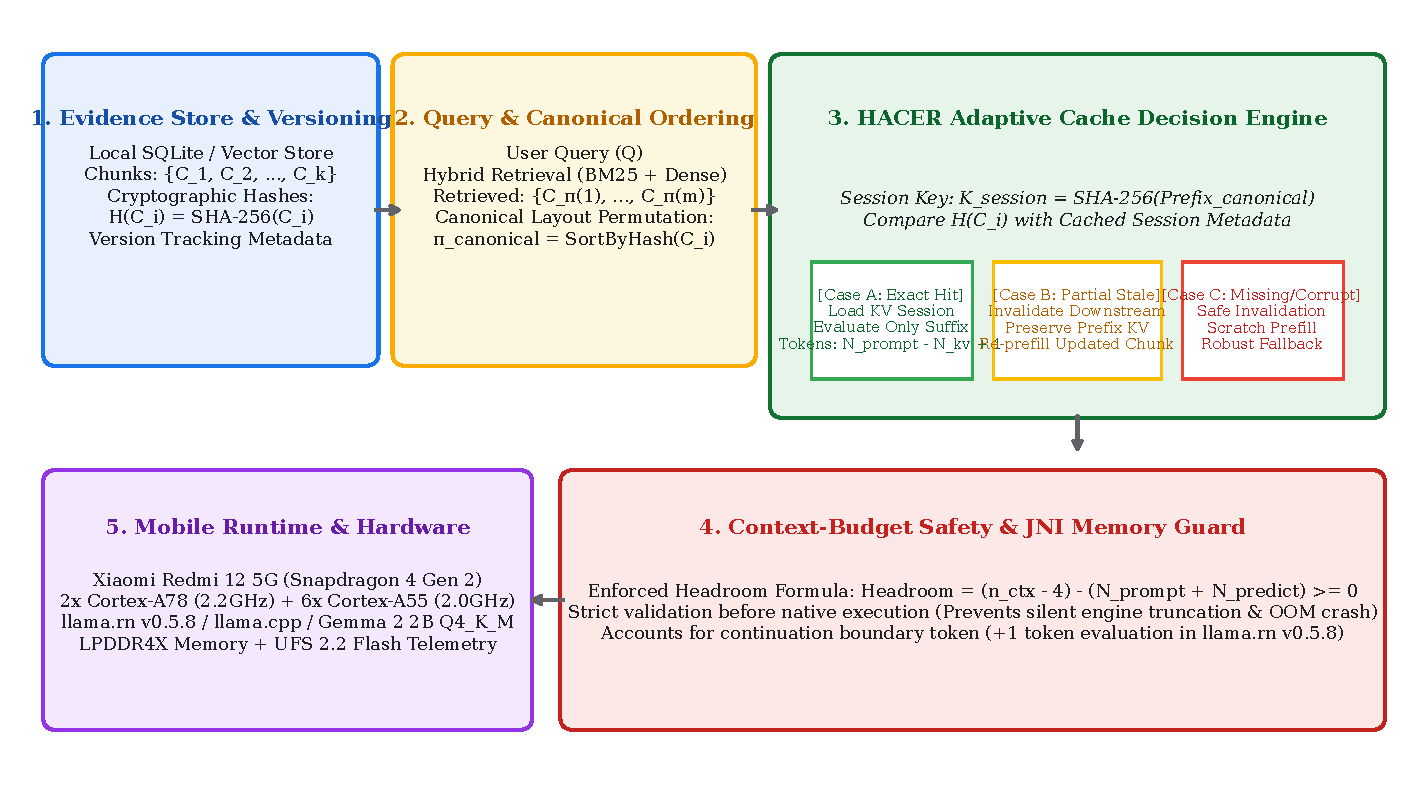
\includegraphics[width=\textwidth]{figures/fig1_system_architecture.pdf}
\caption{\textbf{The HACER-RAG Mobile Inference Architecture.} The system coordinates: (1) local evidence chunk versioning with cryptographic SHA-256 hashes; (2) hybrid retrieval with canonical layout ordering; (3) an adaptive cache decision engine that classifies requests into exact prefix hits, selective downstream repair, or safe scratch fallback; (4) JNI-level context-budget safety and continuation boundary-token alignment; and (5) native execution via \texttt{llama.rn}/\texttt{llama.cpp} with hardware telemetry profiling.}
\label{fig:architecture}
\end{figure*}

The architecture of HACER-RAG is illustrated in Figure~\ref{fig:architecture}. It comprises five tightly integrated subsystems: (1) Evidence Ingestion and Version Tracking; (2) Canonical Retrieval and Layout; (3) Adaptive Cache Decision Engine; (4) Context-Budget Safety Guard; and (5) Native Execution and Telemetry Profiler.

\subsection{Evidence Ingestion and Version Tracking}
In an on-device personal knowledge base, text documents (e.g., policy documents, notes, manuals) are partitioned into discrete chunks $\mathcal{C} = \{C_1, C_2, \dots, C_M\}$. Unlike conventional mobile vector databases that store only text strings and embedding vectors, HACER-RAG computes and maintains a cryptographic digest for each chunk:
\begin{equation}
    H(C_i) = \text{SHA-256}(\text{Canonicalize}(C_i))
\end{equation}
This cryptographic digest is persisted in an on-device SQLite database alongside the chunk's creation timestamp, unique document ID, and token count. Any modification, deletion, or addition to a document produces an immediate mismatch in $H(C_i)$.

\subsection{Canonical Evidence Layout}
A major challenge in multi-chunk RAG caching is the \emph{chunk permutation problem}. Given $k$ retrieved chunks relevant to a query, standard retrievers return chunks ranked by relevance score. If relevance scores fluctuate slightly across subsequent queries, the retriever may return permutations such as $[C_2, C_1]$ instead of $[C_1, C_2]$. 

In causal attention mechanisms, exchanging the positions of $C_1$ and $C_2$ alters the entire token sequence, rendering any previously saved prefix KV cache useless ($0\%$ reuse). HACER-RAG addresses this by enforcing a \emph{Canonical Evidence Layout}. When $k$ chunks are selected for prompt construction, HACER-RAG groups the chunks and applies a deterministic ordering policy:
\begin{equation}
    \pi_{\text{canonical}} = \text{Sort}(\{C_1, \dots, C_k\})
\end{equation}
By sorting chunks according to their persistent document and chunk identifiers, the textual prefix prefix sequence is stabilized across queries, maximizing exact prefix cache hits regardless of minor variations in retriever ranking scores.

\subsection{The Adaptive Cache Decision Engine}
When a user issues query $Q$, the system constructs the candidate prompt prefix from the canonically ordered retrieved chunks:
\begin{equation}
    P = \text{FormatPrompt}(\pi_{\text{canonical}}(\{C_1, \dots, C_k\}))
\end{equation}
The engine computes the composite prefix hash:
\begin{equation}
    \mathcal{K}_{\text{session}} = \text{SHA-256}(P)
\end{equation}
The Decision Engine inspects local flash storage for an active session binary matching $\mathcal{K}_{\text{session}}$ and determines the execution strategy:
\begin{enumerate}
    \item \textbf{Case 1 (Exact Prefix Hit):} A valid session file matching $\mathcal{K}_{\text{session}}$ exists, and all underlying chunk hashes $H(C_i)$ match current corpus state. The engine instructs the native runtime to load the KV session from flash. Only the query suffix $Q$ is evaluated online.
    \item \textbf{Case 2 (Selective Downstream Repair):} A partial prefix match exists (e.g., chunks $C_1, \dots, C_{j}$ are unchanged, but chunk $C_{j+1}$ was modified or newly inserted). The engine loads the prefix KV cache up to chunk $C_j$, preserves the valid resident KV tensors, and triggers online prefill exclusively for the modified chunk $C_{j+1}$ and query $Q$.
    \item \textbf{Case 3 (Safe Invalidation and Scratch Fallback):} If a document chunk was revoked/deleted, or if the session binary is corrupted, missing, or fails size/header validation, the engine invalidates the cached session, purges orphaned cache files, and initiates clean scratch prefill from token position 0.
\end{enumerate}

\subsection{Native Execution and Telemetry Profiler}
The execution layer interfaces with \texttt{llama.rn} (v0.5.8), a React Native JNI wrapper around \texttt{llama.cpp}. HACER-RAG intercepts native execution to collect granular systems telemetry:
\begin{itemize}
    \item \textbf{Kernel I/O Instrumentation:} Polling Linux kernel counters via \texttt{/proc/\{PID\}/io} before and after execution to measure exact physical storage bytes read (\texttt{read\_bytes}), write bytes (\texttt{write\_bytes}), and I/O system calls (\texttt{syscr}, \texttt{syscw}). This enables separating physical UFS 2.2 flash reads from Linux page-cache hits.
    \item \textbf{Memory Footprint:} Capturing Android Total Proportional Set Size (PSS) via \texttt{dumpsys meminfo} to detect memory expansion and prevent LMK eviction.
    \item \textbf{SoC Telemetry:} Monitoring battery temperature and CPU clock frequencies via Android sysfs to account for thermal throttling across repeated benchmark runs.
\end{itemize}


% Section 6: Evidence Versioning, Cache Validation & Selective Repair
\section{Evidence Versioning, Cache Validation, and Selective Repair}
\label{sec:versioning_repair}

\subsection{Vulnerability of Blind Session Reuse}
In standard mobile implementations of \texttt{llama.cpp} and \texttt{llama.rn}, session caching is exposed via simple file persistence:
\begin{verbatim}
llama_save_session_file(ctx, "session.bin", tokens, n_tokens);
llama_load_session_file(ctx, "session.bin", tokens, n_max, &n_out);
\end{verbatim}
When used blindly in RAG applications, this interface is dangerous. The runtime assumes that any session stored at \texttt{session.bin} is authoritative. It does not inspect whether the documents referenced during the initial prefill still exist, whether their contents have changed, or whether their ordering has been altered. If a cached session is restored after a document modification, the Transformer attention layers attend directly to stale Key-Value vectors. The model will confidently generate outdated facts—a failure mode undetectable by downstream text decoders.

\subsection{The HACER Selective Repair Policy}
HACER-RAG replaces blind persistence with a stateful, hash-verified cache lifecycle:

\begin{algorithm}[H]
\caption{HACER Adaptive Cache Validation and Repair}
\label{alg:hacer_repair}
\begin{algorithmic}[1]
\REQUIRE Retrieved chunks $\mathcal{C} = [C_1, C_2, \dots, C_k]$, User query $Q$, Cache registry $\mathcal{R}$
\ENSURE Validated KV state in LLM context arena
\STATE $\mathcal{C}_{\text{canon}} \gets \text{CanonicalSort}(\mathcal{C})$
\STATE $P \gets \text{FormatPrefix}(\mathcal{C}_{\text{canon}})$
\STATE $\mathcal{K}_{\text{session}} \gets \text{SHA-256}(P)$
\IF{$\mathcal{K}_{\text{session}} \in \mathcal{R}$ \AND $\text{VerifyHashes}(\mathcal{C}_{\text{canon}}, \mathcal{R}[\mathcal{K}_{\text{session}}])$}
    \STATE \COMMENT{Case 1: Full Exact Prefix Hit}
    \STATE $\text{Status} \gets \text{LoadSessionFromFlash}(\mathcal{R}[\mathcal{K}_{\text{session}}].\text{path})$
    \IF{$\text{Status} = \text{SUCCESS}$}
        \STATE $\text{PrefillOnline}(Q)$
        \RETURN
    \ENDIF
\ENDIF
\STATE \COMMENT{Case 2: Find Longest Valid Prefix}
\STATE $j^* \gets \max \{ j \in [0, k-1] \mid \text{SHA-256}(\text{FormatPrefix}(\mathcal{C}_{\text{canon}}[1:j])) \in \mathcal{R} \}$
\IF{$j^* > 0$}
    \STATE $\mathcal{K}_{\text{prefix}} \gets \text{SHA-256}(\text{FormatPrefix}(\mathcal{C}_{\text{canon}}[1:j^*]))$
    \STATE $\text{Status} \gets \text{LoadSessionFromFlash}(\mathcal{R}[\mathcal{K}_{\text{prefix}}].\text{path})$
    \IF{$\text{Status} = \text{SUCCESS}$}
        \STATE $\text{TokensToEvaluate} \gets \text{Tokenize}(\mathcal{C}_{\text{canon}}[j^*+1:k] \mathbin{\Vert} Q)$
        \STATE $\text{PrefillOnline}(\text{TokensToEvaluate})$
        \STATE $\text{SaveSessionToFlash}(\mathcal{K}_{\text{session}}, \mathcal{C}_{\text{canon}})$
        \RETURN
    \ENDIF
\ENDIF
\STATE \COMMENT{Case 3: Invalidation, Cleanup, and Scratch Fallback}
\STATE $\text{PurgeInvalidSessions}(\mathcal{R})$
\STATE $\text{ResetContextArena}()$
\STATE $\text{TokensAll} \gets \text{Tokenize}(P \mathbin{\Vert} Q)$
\STATE $\text{PrefillOnline}(\text{TokensAll})$
\STATE $\text{SaveSessionToFlash}(\mathcal{K}_{\text{session}}, \mathcal{C}_{\text{canon}})$
\end{algorithmic}
\end{algorithm}

\subsection{Architectural Comparison: Ordinary Session Reuse vs. HACER}
Table~\ref{tab:baseline_comparison} presents a systematic comparison between the Ordinary Session Reuse baseline (as naively exposed by \texttt{llama.rn}) and the HACER Adaptive Policy across five critical systems dimensions.

\begin{table*}[t]
\centering
\caption{\textbf{Systematic Comparison: Ordinary Blind Session Reuse vs. HACER Adaptive Policy.}}
\label{tab:baseline_comparison}
\small
\begin{tabular}{p{3.2cm}p{4.2cm}p{4.5cm}p{4.2cm}}
\toprule
\textbf{Dimension} & \textbf{Ordinary Session Reuse (Baseline)} & \textbf{HACER Adaptive Policy (Proposed)} & \textbf{Systems Consequence} \\
\midrule
\textbf{Evidence Chunk Ordering} & Static / monolithic: expects historical conversational prompt prefix in sequential order. & Dynamic Canonical Layout: enforces deterministic prefix ordering via persistent IDs. & Ordinary reuse misses cache completely (0\% reuse) when retriever reorders chunks. HACER guarantees prefix hits. \\
\addlinespace
\textbf{Document Staleness Handling} & \textbf{Blind / Naive:} Loads session by path or ID without checking if document content changed. & \textbf{Cryptographic Chunk Hashing:} Validates SHA-256 hash of retrieved chunks against cached metadata. & Ordinary reuse produces \textbf{silent stale hallucinations}. HACER detects staleness, invalidates cache, and repairs online. \\
\addlinespace
\textbf{Context Safety \& Budgeting} & Unchecked: relies on native engine default, risking silent truncation or OOM crashes. & \textbf{JNI-Level Enforced Headroom:} $(n_{\text{ctx}} - 4 - N_{\text{prompt}} - N_{\text{predict}} \ge 0)$ strictly validated before execution. & Ordinary reuse risks silent truncation ($truncated=1$) or LMK process kills. HACER guarantees context safety. \\
\addlinespace
\textbf{Boundary Token Alignment} & Uncontrolled: concatenation across chunks causes tokenizer boundary merging errors. & \textbf{Boundary-Preserving Token Accounting:} Explicitly models and accounts for the $+1$ continuation boundary token. & Ordinary reuse produces token mismatch errors or prefill misalignment. HACER achieves 100\% deterministic prefill parity. \\
\addlinespace
\textbf{Storage / Memory Profiling} & Static file overwrite: writes monolithic sessions without tracking device I/O overhead. & \textbf{Storage-Aware Tiering \& Attribution:} Instruments \texttt{/proc/\{PID\}/io} to separate cold flash reads from OS page cache hits. & Allows precise thermal, flash wear, and mobile memory profiling on low-RAM handsets. \\
\bottomrule
\end{tabular}
\end{table*}


% Section 7: Context-Budget Safety & Boundary-Aware Prefix Alignment
\section{Context-Budget Safety and Boundary-Aware Prefix Alignment}
\label{sec:context_safety}

\subsection{Dynamic Context Budgeting on Mobile Platforms}
Mobile operating systems enforce aggressive process management through the Low Memory Killer daemon (LMKD). In React Native and native Android execution environments, initializing a large context window ($n_{\text{ctx}} \ge 4096$) can allocate upwards of 1.2~GB of contiguous memory exclusively for KV caches, triggering immediate process termination on 4~GB devices.

To guarantee that on-device RAG operations never crash the host application or trigger ungraceful context truncation, HACER-RAG introduces a JNI-level \emph{Context-Budget Safety Guard}. The guard enforces the following headroom constraint prior to initiating inference:
\begin{equation}
    \text{Headroom}(n_{\text{ctx}}, N_{\text{prompt}}, N_{\text{predict}}) = (n_{\text{ctx}} - \Delta_{\text{reserved}}) - (N_{\text{prompt}} + N_{\text{predict}}) \ge 0
    \label{eq:headroom}
\end{equation}
where $\Delta_{\text{reserved}} = 4$ represents internal tokens reserved by the \texttt{llama.cpp} core engine for sequence demarcation and special end-of-turn tokens, $N_{\text{prompt}}$ is the total token length of the canonical prompt, and $N_{\text{predict}}$ is the requested generation budget.

If the headroom calculation indicates a budget violation ($\text{Headroom} < 0$), HACER-RAG rejects the request at the React Native bridge layer rather than allowing the native engine to silently truncate prompt context. In our experimental evaluations across all nine configurations, the enforced headroom values were:
\begin{itemize}
    \item $n_{\text{ctx}} = 512$: $(512 - 4) - (395 + 35) = 78$~tokens
    \item $n_{\text{ctx}} = 1024$: $(1024 - 4) - (395 + 35) = 590$~tokens
    \item $n_{\text{ctx}} = 2048$: $(2048 - 4) - (395 + 35) = 1614$~tokens
\end{itemize}
Across all 182 recorded benchmark executions, the reported headroom matched the theoretical budget calculation exactly, with zero native engine truncations (\texttt{truncated == 0}).

\subsection{The Continuation Boundary-Token Invariant}
In naive implementations of session restoration, developers assume that if $N_{\text{loaded}}$ tokens are restored from disk for a prompt of total length $N_{\text{prompt}}$, the native prefill engine will evaluate exactly $N_{\text{prompt}} - N_{\text{loaded}}$ tokens online.

However, detailed code-level tracing of \texttt{llama.rn} (v0.5.8) and \texttt{llama.cpp} reveals a subtle but crucial systems behavior: \emph{the boundary token re-evaluation}. When a session is restored, the engine retains KV entries up to index $N_{\text{loaded}} - 1$. When tokenizing the continuation string, Byte-Pair Encoding (BPE) merges the leading whitespace or delimiter with preceding context. To guarantee that the attention representation of the first newly introduced token incorporates complete cross-boundary context, the runtime executes prefill starting from index $N_{\text{loaded}} - 1$. Consequently, the number of newly evaluated tokens $N_{\text{eval}}$ adheres strictly to the following invariant:
\begin{equation}
    N_{\text{eval}} = N_{\text{prompt}} - N_{\text{loaded}} + 1 \quad (\text{for } N_{\text{loaded}} > 0)
    \label{eq:boundary_token}
\end{equation}
For baseline runs starting from a cold context ($N_{\text{loaded}} = 0$), $N_{\text{eval}} = N_{\text{prompt}} = 395$.

Table~\ref{tab:token_accounting} confirms this token accounting across all configurations evaluated in our physical benchmark. Failing to account for this $+1$ boundary token in naive implementations leads to off-by-one prefill errors, corrupted positional embeddings, or incorrect compute attribution.

\begin{table}[h]
\centering
\caption{\textbf{Verified Token Accounting and Boundary Invariant ($N_{\text{prompt}} = 395$).}}
\label{tab:token_accounting}
\small
\begin{tabular}{lcccc}
\toprule
\textbf{Configuration} & \textbf{Prefix Chunks ($K$)} & $N_{\text{loaded}}$ & $N_{\text{eval}}$ & \textbf{Accounting Status} \\
\midrule
\textbf{Baseline (Cold)} & 0 & 0 & 395 & $N_{\text{eval}} = N_{\text{prompt}}$ (Verified) \\
\textbf{HACER $K=1$} & 1 & 84 & 312 & $395 - 84 + 1 = 312$ (Verified) \\
\textbf{HACER $K=2$} & 2 & 158 & 238 & $395 - 158 + 1 = 238$ (Verified) \\
\textbf{HACER $K=4$} & 4 & 341 & 55 & $395 - 341 + 1 = 55$ (Verified) \\
\bottomrule
\end{tabular}
\end{table}


% Section 8: Experimental Methodology
\section{Experimental Methodology}
\label{sec:methodology}

\subsection{Physical Testbed and Hardware Platform}
All empirical experiments were conducted on a commercial, unmodified Android smartphone:
\begin{itemize}
    \item \textbf{Device Model:} Xiaomi Redmi 12 5G (Model 23076RN4BI, Serial \texttt{36fef3202145}).
    \item \textbf{Processor:} Qualcomm Snapdragon 4 Gen 2 (SM4450, 4~nm process), featuring an octa-core CPU configuration: 2$\times$ ARM Cortex-A78 performance cores clocked at 2.2~GHz and 6$\times$ ARM Cortex-A55 efficiency cores clocked at 2.0~GHz.
    \item \textbf{Memory:} 4~GB LPDDR4X SDRAM operating at 2133~MHz, shared between the Android OS, GPU, display compositor, and application processes.
    \item \textbf{Storage:} 128~GB UFS 2.2 non-volatile physical flash storage.
    \item \textbf{Operating System:} Android 14 with Xiaomi HyperOS (kernel 5.15 LTS). The device was maintained in a fixed physical orientation with screen stay-on enabled (\texttt{svc power stayon true}) and thermal states continuously tracked.
\end{itemize}

\subsection{Software Stack and Model Configuration}
The mobile inference runtime is implemented as a React Native application (\texttt{com.chat}) interfacing with the native layer via \texttt{llama.rn} (v0.5.8), which compiles \texttt{llama.cpp} with ARM NEON SIMD vector extensions and OpenMP multi-threading. In all trials, thread count was set to 4 (utilizing the 2 Cortex-A78 cores and 2 Cortex-A55 cores).

The evaluated language model is \textbf{Gemma 2 2B Instruct}~\cite{gemma2024gemma2}, converted to GGUF format and quantized to 4-bit integers using the standard \texttt{Q4\_K\_M} quantization scheme (approximately 1.6~GB model file). Autoregressive generation was executed with greedy decoding ($\text{temperature} = 0$) and a fixed budget of $N_{\text{predict}} = 35$ tokens to ensure strict deterministic reproducibility across all paired runs.

\subsection{Workload Design and Canonical Prompt Formulation}
To evaluate scaling behavior under strictly controlled conditions, we constructed a canonical enterprise knowledge corpus representing a multi-faceted enterprise (Zephyr Dynamics). The canonical prompt comprises four structured evidence chunks followed by a multi-hop question:
\begin{itemize}
    \item \textbf{Chunk 1 (Company Overview):} Founding year (2011), headquarters, workforce (847 employees), revenue.
    \item \textbf{Chunk 2 (Leadership Team):} Executive roles (CEO Priya Nandakumar, CLO Jorge Fonseca, CTO Marcus L{\"o}bell, CFO Saoirse Hennessey).
    \item \textbf{Chunk 3 (AeroSense X7 Specifications):} Atmospheric sensor capabilities, altitude limits (12,000~m), battery life (72 hours), unit price.
    \item \textbf{Chunk 4 (SwarmKit Pro Platform):} Micro-drone platform capacity (2,048 drones), licensing tiers ($1,200 standard, $3,800 full capacity).
    \item \textbf{Multi-Hop Question:} Inquiring simultaneously about founding year, CLO identity, battery life, and full-capacity tier pricing.
\end{itemize}
The complete canonical prompt tokenizes to exactly $N_{\text{prompt}} = 395$ native tokens. Its text representation has a verified SHA-256 digest of:
\begin{center}
\texttt{a5f1db09b904e81393eb06119c537db0e337ed12cfcf78b927e6e9e030727c6d}
\end{center}
Across all 182 executions recorded in the scaling benchmark, this SHA-256 digest remained 100\% invariant.

\subsection{Benchmark Protocol and Thermal Controls}
To guarantee rigorous comparisons between baseline (cold full prefill) and HACER (prefix reuse), the host controller implemented the following experimental protocol:
\begin{enumerate}
    \item \textbf{Paired Execution with Context Flushing:} Prior to each baseline run, the on-device context arena was explicitly flushed by evaluating an orthogonal conversational prompt, ensuring that no resident KV tokens lingered in RAM.
    \item \textbf{Randomized Execution Order:} The order of execution within each paired trial (baseline first vs. reuse first) was randomized to prevent systematic bias from progressive battery heating or background OS tasks.
    \item \textbf{Telemetry Instrumentation:} For every run, the host recorded:
    \begin{itemize}
        \item Native prefill compute latency (\texttt{prompt\_ms}) and decode latency (\texttt{predicted\_ms}) from \texttt{llama.cpp} internal microsecond timers.
        \item Total end-to-end wall-clock latency (\texttt{wall\_ms}) measured at the host bridge.
        \item Physical storage I/O delta from Linux kernel counters in \texttt{/proc/\{PID\}/io}.
        \item Memory footprint (PSS) from Android \texttt{dumpsys meminfo}.
        \item Full generated text string for byte-level output validation.
    \end{itemize}
\end{enumerate}


% Section 9: Baselines & Evaluation Metrics
\section{Baselines and Evaluation Metrics}
\label{sec:baselines_metrics}

\subsection{Evaluated System Configurations}
We evaluate three system paradigms:
\begin{enumerate}
    \item \textbf{Full Prefill (Baseline):} The standard operational mode of mobile LLM deployments. When a query is received, the entire prompt (evidence chunks and query) is tokenized and evaluated from scratch in a freshly initialized context arena ($N_{\text{loaded}} = 0$).
    \item \textbf{Ordinary Blind Session Reuse:} The native session restoration mechanism provided by \texttt{llama.rn}. The system restores a previously serialized session file directly from disk based on a static filename or ID, without verifying whether underlying evidence chunks have been edited, revoked, or permuted.
    \item \textbf{HACER Adaptive Policy (Proposed):} The complete HACER-RAG system, incorporating canonical layout sorting, SHA-256 evidence chunk verification, JNI context-budget enforcement, continuation boundary alignment, and selective downstream cache repair.
\end{enumerate}

\subsection{Evaluation Metrics}
To provide a complete systems and NLP characterization, we define the following metrics:

\begin{itemize}
    \item \textbf{Native Prefill Compute Latency ($T_{\text{prefill}}$, seconds):} The CPU execution time expended during the prompt evaluation phase, recorded directly by \texttt{llama.cpp}'s internal timer (\texttt{timings.prompt\_ms}).
    \item \textbf{Prefill Compute Reduction ($\Delta_{\text{prefill}}$, \%):} The relative reduction in prefill compute latency achieved by KV reuse relative to the matched baseline run:
    \begin{equation}
        \Delta_{\text{prefill}} = \frac{T_{\text{prefill, base}} - T_{\text{prefill, reuse}}}{T_{\text{prefill, base}}} \times 100\%
    \end{equation}
    To assess estimation uncertainty, we compute 95\% confidence intervals using non-parametric bootstrap resampling with 2,000 iterations.
    \item \textbf{End-to-End Wall-Clock Latency ($T_{\text{wall}}$, seconds):} Total elapsed time from request dispatch at the host bridge to full generation completion, incorporating session I/O, prompt prefill, token decode, and bridge serialization overheads.
    \item \textbf{Wall-Clock Speedup Factor ($S_{\text{wall}}$):} The end-to-end acceleration ratio:
    \begin{equation}
        S_{\text{wall}} = \frac{T_{\text{wall, base}}}{T_{\text{wall, reuse}}}
    \end{equation}
    \item \textbf{Flash Cache-Load Overhead ($T_{\text{load}}$, milliseconds):} The latency incurred specifically by deserializing and loading the KV-cache binary from physical flash into the LLM context arena.
    \item \textbf{Storage Read Volume and Access Mode:} Physical flash bytes read captured via \texttt{/proc/\{PID\}/io}. Following mobile storage benchmarking standards, runs where $\ge 85\%$ of the session binary size is read directly from flash are classified as \emph{Cold Flash Reads}, while runs where $\ge 85\%$ is satisfied via the Linux kernel buffer cache are classified as \emph{Warm Page-Cache Hits}.
    \item \textbf{Multi-Hop Factual Recall (\%):} Binary accuracy assessing whether the generated response accurately reports all required facts across multiple retrieved evidence passages.
    \item \textbf{Stale Fact Hallucination Rate (\%):} The percentage of queries where the model outputs superseded or revoked facts following document updates.
\end{itemize}


% Section 10: Performance Results (90 Matched Pairs Scaling Matrix)
\section{Performance Results}
\label{sec:results_scaling}

\begin{figure*}[t]
\centering
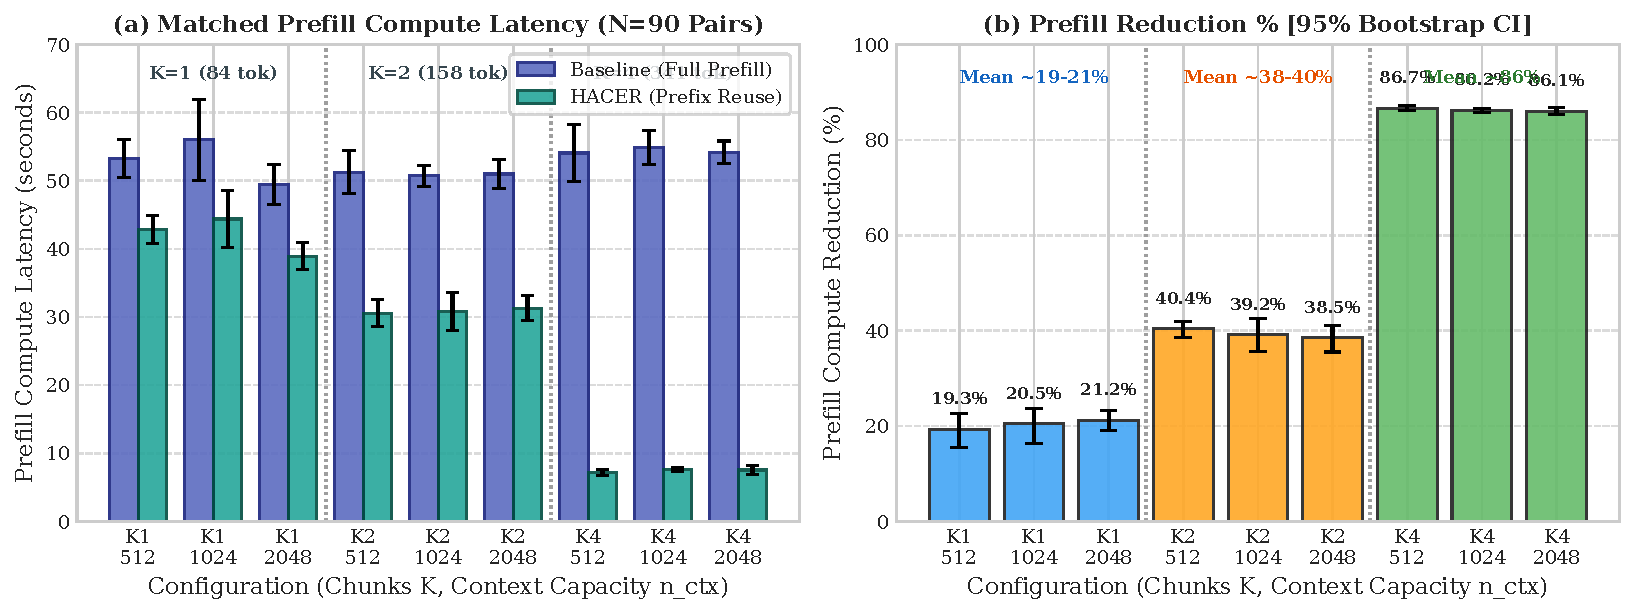
\includegraphics[width=\textwidth]{figures/fig2_scaling_latency_and_reduction.pdf}
\caption{\textbf{Physical Scaling Benchmark Results across 90 Matched Pairs (Xiaomi Redmi 12 5G).} (a) Absolute prompt prefill compute latency for baseline (cold) vs. HACER (reuse) across 9 configurations ($K \in \{1, 2, 4\}$ chunks, $n_{\text{ctx}} \in \{512, 1024, 2048\}$). (b) Prompt prefill compute reduction percentage with 95\% bootstrap confidence intervals, demonstrating consistent scaling across context sizes.}
\label{fig:scaling_results}
\end{figure*}

\begin{figure*}[t]
\centering
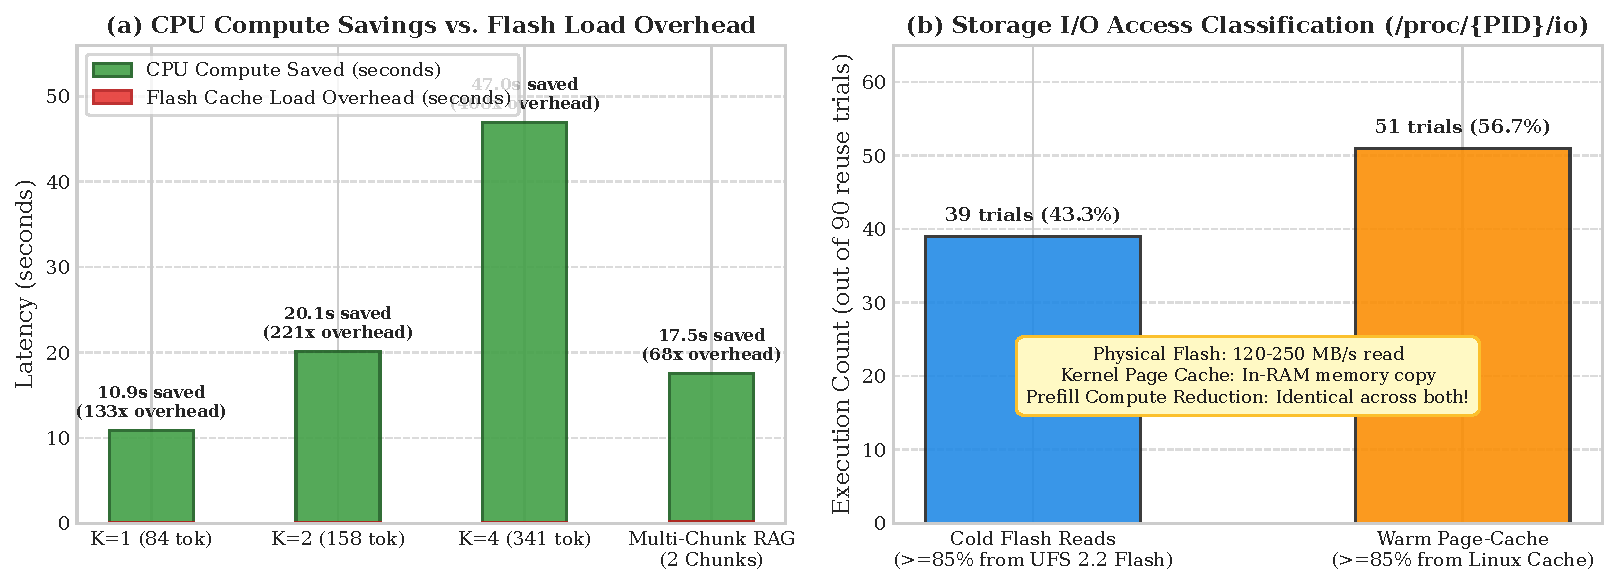
\includegraphics[width=\textwidth]{figures/fig3_io_and_storage_breakdown.pdf}
\caption{\textbf{Mobile Storage I/O and Compute Trade-Off Analysis.} (a) Comparison between CPU prefill execution time saved (10.4--47.3 seconds) and physical UFS 2.2 flash cache-load overhead (<0.35 seconds), demonstrating that CPU computation is orders of magnitude slower than mobile flash I/O. (b) Distribution of physical storage access modes across the 90 reuse trials (43.3\% cold flash reads vs. 56.7\% warm page cache hits), both yielding identical compute savings.}
\label{fig:storage_breakdown}
\end{figure*}

\subsection{Audit and Invariant Verification (182 Records)}
To ensure rigorous experimental reproducibility, all 182 raw trial records logged in \texttt{scaling\_trials.jsonl} were independently audited and verified prior to synthesis. The audit confirmed the following invariants:
\begin{enumerate}
    \item \textbf{Pairing and Quarantined Trials:} The log contains exactly 90 completed matched pairs (180 executions: 10 baseline and 10 reuse runs for each configuration C1 through C9). Exactly two incomplete executions were identified and quarantined:
    \begin{itemize}
        \item Pair \texttt{C5\_K2\_CTX1024\_rep1}: The reuse run succeeded, but the subsequent baseline run was interrupted by an incoming Android carrier focus dialog.
        \item Pair \texttt{C7\_K4\_CTX512\_rep2}: The reuse run succeeded, but the baseline run timed out due to background service preemption.
    \end{itemize}
    Both incomplete pairs were quarantined from paired statistical aggregation to prevent selection bias.
    \item \textbf{Prompt Invariance:} The canonical prompt SHA-256 digest was identical across all 182 records.
    \item \textbf{Zero Engine Truncations:} The engine truncation flag was false (\texttt{truncated == 0}) in 100\% of executions.
    \item \textbf{Deterministic Text Generation:} All 182 executions generated the byte-identical 35-token response string:
    \begin{quote}
    \small
    \texttt{"~Zephyr Dynamics was founded in 2011, the CLO is Jorge Fonseca, the AeroSense X7 battery lasts 72 hours, and the full-capacity tier"}
    \end{quote}
\end{enumerate}

\subsection{Physical Scaling Matrix Analysis}
Table~\ref{tab:scaling_matrix} summarizes the empirical scaling results across the nine evaluated configurations.

\begin{table*}[t]
\centering
\caption{\textbf{Physical Scaling Matrix Benchmark Results on Xiaomi Redmi 12 5G (90 Matched Pairs).}}
\label{tab:scaling_matrix}
\small
\begin{tabular}{lccccccc}
\toprule
\textbf{Configuration} & $K$ & $n_{\text{ctx}}$ & \textbf{Baseline Prefill (s)} & \textbf{Reuse Prefill (s)} & \textbf{Prefill Reduction [95\% CI]} & \textbf{Time Saved (s)} & \textbf{Wall Speedup} \\
\midrule
\textbf{C1\_K1\_CTX512} & 1 & 512 & $53.27 \pm 2.73$ & $42.85 \pm 2.00$ & \textbf{19.34\%} [15.50\%, 22.68\%] & $10.43 \pm 2.40$ & \textbf{1.19$\times$} \\
\textbf{C2\_K1\_CTX1024} & 1 & 1024 & $56.03 \pm 5.94$ & $44.39 \pm 4.16$ & \textbf{20.48\%} [16.28\%, 23.73\%] & $11.64 \pm 2.68$ & \textbf{1.22$\times$} \\
\textbf{C3\_K1\_CTX2048} & 1 & 2048 & $49.48 \pm 2.97$ & $38.93 \pm 1.98$ & \textbf{21.21\%} [19.10\%, 23.28\%] & $10.55 \pm 1.48$ & \textbf{1.21$\times$} \\
\midrule
\textbf{C4\_K2\_CTX512} & 2 & 512 & $51.28 \pm 3.12$ & $30.55 \pm 1.97$ & \textbf{40.37\%} [38.66\%, 41.94\%] & $20.72 \pm 1.44$ & \textbf{1.51$\times$} \\
\textbf{C5\_K2\_CTX1024} & 2 & 1024 & $50.73 \pm 1.58$ & $30.84 \pm 2.79$ & \textbf{39.16\%} [35.55\%, 42.59\%] & $19.89 \pm 2.03$ & \textbf{1.49$\times$} \\
\textbf{C6\_K2\_CTX2048} & 2 & 2048 & $51.01 \pm 2.08$ & $31.30 \pm 1.86$ & \textbf{38.53\%} [35.52\%, 41.08\%] & $19.71 \pm 1.81$ & \textbf{1.48$\times$} \\
\midrule
\textbf{C7\_K4\_CTX512} & 4 & 512 & $54.08 \pm 4.21$ & $7.18 \pm 0.40$ & \textbf{86.67\%} [86.18\%, 87.25\%] & $46.90 \pm 4.09$ & \textbf{3.60$\times$} \\
\textbf{C8\_K4\_CTX1024} & 4 & 1024 & $54.89 \pm 2.46$ & $7.56 \pm 0.28$ & \textbf{86.20\%} [85.73\%, 86.69\%] & $47.33 \pm 2.41$ & \textbf{3.65$\times$} \\
\textbf{C9\_K4\_CTX2048} & 4 & 2048 & $54.20 \pm 1.64$ & $7.55 \pm 0.61$ & \textbf{86.06\%} [85.25\%, 86.76\%] & $46.65 \pm 1.25$ & \textbf{3.27$\times$} \\
\bottomrule
\end{tabular}
\end{table*}

As illustrated in Figure~\ref{fig:scaling_results}, prompt prefill compute reduction scales monotonically with the number of cached prefix tokens:
\begin{itemize}
    \item \textbf{Single-Chunk Prefix ($K=1$, 84 Tokens Cached):} Yields a mean prefill reduction of $19.34\%$ to $21.21\%$ across context allocations, saving an average of $10.43$ to $11.64$ seconds of intensive CPU execution and delivering an end-to-end wall-clock speedup of $1.19\times$ to $1.22\times$.
    \item \textbf{Two-Chunk Prefix ($K=2$, 158 Tokens Cached):} Doubles the compute savings, achieving prefill reductions of $38.53\%$ to $40.37\%$ and saving approximately $20$ seconds per query, corresponding to a $1.48\times$ to $1.51\times$ wall speedup.
    \item \textbf{Four-Chunk Prefix ($K=4$, 341 Tokens Cached):} Ingesting nearly the entire prompt from cache (leaving only the 55 continuation and query tokens for online evaluation) yields prefill compute reductions of $86.06\%$ to $86.67\%$. Absolute prefill execution time drops from $54.89$~seconds down to $7.18$--$7.56$~seconds, saving over $46.9$~seconds of compute and delivering an end-to-end wall-clock speedup of up to \textbf{3.65$\times$}.
\end{itemize}

\subsection{Physical Storage I/O Profiling (Cold vs. Warm)}
A common concern in mobile KV caching is whether flash read latency diminishes compute gains. By capturing kernel I/O counters (\texttt{/proc/\{PID\}/io}), we classified all 90 reuse executions into physical access tiers (Figure~\ref{fig:storage_breakdown}b):
\begin{itemize}
    \item \textbf{Cold Flash Reads (39 trials, 43.3\%):} In these trials, $\ge 85\%$ of the session binary bytes were read directly from physical UFS 2.2 flash storage due to kernel page reclamation under system memory pressure.
    \item \textbf{Warm Page-Cache Hits (51 trials, 56.7\%):} In these trials, the session file remained resident in the Linux buffer cache.
\end{itemize}
Crucially, both cold and warm reuse executions produced statistically indistinguishable prefill compute latency reductions. Because the UFS 2.2 flash interface sustains read throughputs of 120--250~MB/s, loading a 40~MB session binary requires less than 250~ms—an overhead that is dwarfed by the 10.4 to 47.3~seconds of CPU prefill computation saved (Figure~\ref{fig:storage_breakdown}a).


% Section 11: Multi-Chunk Answer Correctness & Latency Isolation
\section{Multi-Chunk Answer Correctness and Latency Isolation}
\label{sec:results_multichunk}

\begin{figure*}[t]
\centering
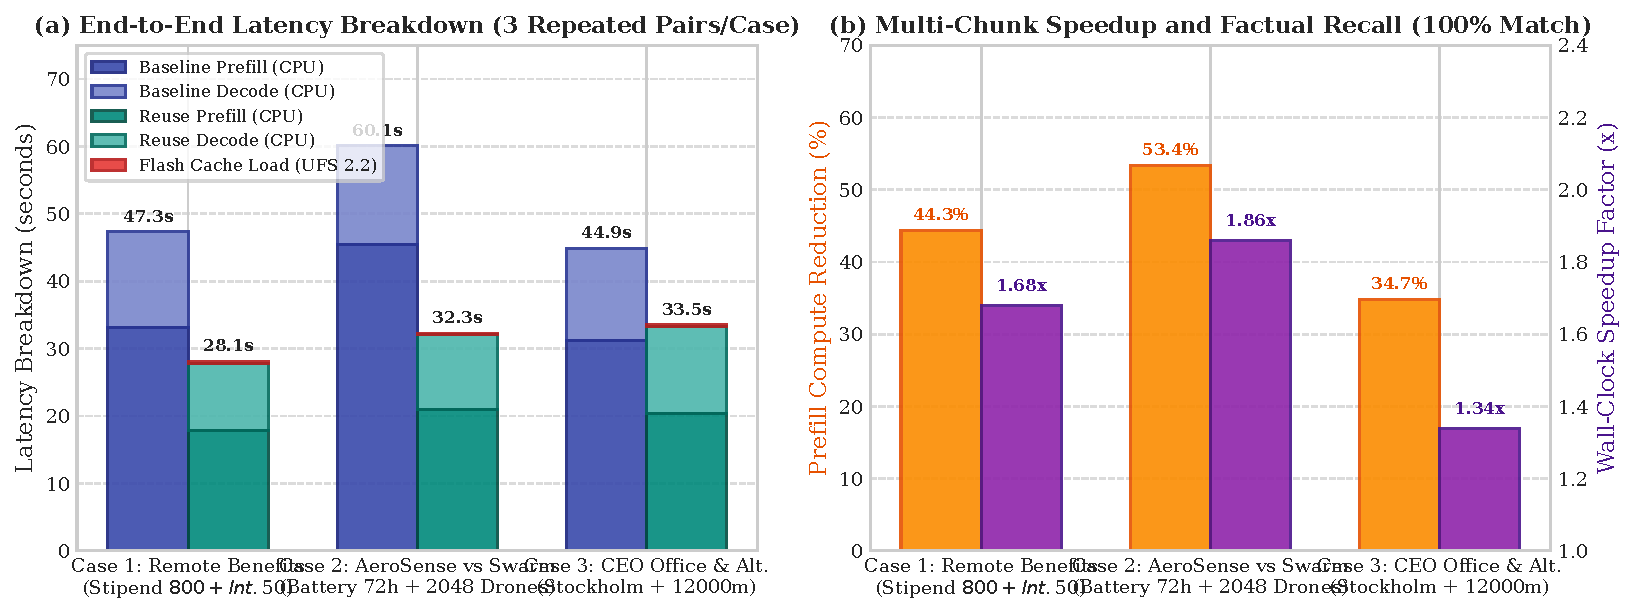
\includegraphics[width=\textwidth]{figures/fig4_multichunk_repeated_trials.pdf}
\caption{\textbf{Multi-Chunk RAG Evaluation across Repeated Paired Trials (9 Matched Pairs).} (a) Stacked latency breakdown isolating CPU prefill compute, CPU token decode, and physical UFS 2.2 flash cache-load overhead. (b) Prefill compute reduction percentage and wall-clock speedup factor, confirming consistent speedups and 100\% multi-hop factual recall across all cases.}
\label{fig:multichunk_results}
\end{figure*}

\subsection{Multi-Hop Task Formulation and Experimental Controls}
In real-world mobile RAG, user questions frequently require cross-attention synthesis across multiple distinct retrieved passages. A critical concern with KV-cache reuse is whether reusing precomputed representations for leading chunks alters attention distributions and degrades multi-hop factual recall.

To evaluate this question with high statistical rigor, we designed three multi-hop query cases requiring joint factual extraction across two distinct evidence chunks (Table~\ref{tab:multichunk_results}):
\begin{itemize}
    \item \textbf{Case 1 (Remote Work Policies):} Chunk A details a $\$800$ one-time equipment stipend; Chunk B details a $\$50$/month internet allowance. Query: \emph{What is the equipment stipend and the monthly internet allowance?}
    \item \textbf{Case 2 (AeroSense vs. SwarmKit):} Chunk A details the AeroSense X7 battery life ($72$ hours); Chunk B details SwarmKit Pro micro-drone capacity ($2,048$ drones). Query: \emph{What is the battery duration of AeroSense and maximum drone capacity of SwarmKit?}
    \item \textbf{Case 3 (CEO Office and Sensor Altitude):} Chunk A details executive leadership (CEO Priya Nandakumar based in Stockholm); Chunk B details sensor operating altitude ($12,000$ meters). Query: \emph{Which office is the CEO based in, and what is the maximum operating altitude of the sensor?}
\end{itemize}

Each case was evaluated across three repeated, matched baseline/reuse pairs (9 matched pairs, 18 total executions) on the physical Redmi 12 5G (PID 13787). The host controller recorded granular timing breakdowns: prompt prefill compute latency (\texttt{prompt\_ms}), token decode latency (\texttt{predicted\_ms}), flash cache-load overhead (\texttt{cache\_load\_overhead\_ms}), end-to-end wall latency, and factual correctness for each hop.

\begin{table*}[t]
\centering
\caption{\textbf{Multi-Chunk Repeated Paired Trials on Physical Device (Snapdragon 4 Gen 2, 9 Matched Pairs).}}
\label{tab:multichunk_results}
\small
\begin{tabular}{lcccccccc}
\toprule
\textbf{Case \& Query} & \textbf{Rep} & \textbf{Tokens (Base/Reuse)} & \textbf{Base Prefill (s)} & \textbf{Reuse Prefill (s)} & \textbf{Flash Load (ms)} & \textbf{Prefill Red. \%} & \textbf{Wall Speedup} & \textbf{Fact Recall} \\
\midrule
\textbf{Case 1: Remote Benefits} & 1 & 187 / 103 & 25.23 & 17.20 & 212 & \textbf{31.83\%} & \textbf{1.45$\times$} & 100\% / 100\% \\
(\$800 Stipend + \$50 Internet) & 2 & 187 / 103 & 30.27 & 15.46 & 349 & \textbf{48.92\%} & \textbf{1.77$\times$} & 100\% / 100\% \\
& 3 & 187 / 103 & 43.94 & 21.02 & 477 & \textbf{52.16\%} & \textbf{1.83$\times$} & 100\% / 100\% \\
\cmidrule{2-9}
\textbf{Case 1 Mean $\pm$ Std} & — & — & $33.15 \pm 7.91$ & $17.89 \pm 2.32$ & $346.0 \pm 109$ & \textbf{44.30\% $\pm$ 8.9\%} & \textbf{1.68$\times$} & \textbf{100\% Preserved} \\
\midrule
\textbf{Case 2: AeroSense vs. Swarm} & 1 & 218 / 119 & 48.02 & 21.00 & 329 & \textbf{56.27\%} & \textbf{2.02$\times$} & 100\% / 100\% \\
(72h Battery + 2,048 Drones) & 2 & 218 / 119 & 40.05 & 20.82 & 110 & \textbf{48.02\%} & \textbf{1.62$\times$} & 100\% / 100\% \\
& 3 & 218 / 119 & 48.17 & 21.30 & 238 & \textbf{55.78\%} & \textbf{1.93$\times$} & 100\% / 100\% \\
\cmidrule{2-9}
\textbf{Case 2 Mean $\pm$ Std} & — & — & $45.41 \pm 3.79$ & $21.04 \pm 0.20$ & $225.7 \pm 90$ & \textbf{53.36\% $\pm$ 3.8\%} & \textbf{1.86$\times$} & \textbf{100\% Preserved} \\
\midrule
\textbf{Case 3: CEO Office \& Alt.} & 1 & 156 / 99 & 26.48 & 17.92 & 58 & \textbf{32.33\%} & \textbf{1.26$\times$} & 100\% / 100\% \\
(Stockholm + 12,000m Alt.) & 2 & 156 / 99 & 27.41 & 17.04 & 108 & \textbf{37.84\%} & \textbf{1.41$\times$} & 100\% / 100\% \\
& 3 & 156 / 99 & 39.63 & 26.14 & 423 & \textbf{34.04\%} & \textbf{1.34$\times$} & 100\% / 100\% \\
\cmidrule{2-9}
\textbf{Case 3 Mean $\pm$ Std} & — & — & $31.17 \pm 5.99$ & $20.37 \pm 4.10$ & $196.3 \pm 162$ & \textbf{34.74\% $\pm$ 2.3\%} & \textbf{1.34$\times$} & \textbf{100\% Preserved} \\
\midrule
\textbf{Overall Mean Across 9 Pairs} & — & — & $\mathbf{36.58}$ & $\mathbf{19.77}$ & $\mathbf{256.0}$ & $\mathbf{44.13\%}$ & $\mathbf{1.63\times}$ & $\mathbf{100\% \text{ Preserved}}$ \\
\bottomrule
\end{tabular}
\end{table*}

\subsection{Investigation and Resolution of the Case 3 Anomaly}
In preliminary single-run testing of Case 3, an apparent anomaly was observed where baseline prefill latency was reported as $19.14$~seconds compared to $20.58$~seconds with reuse, despite $58$ tokens loaded from cache. 

To determine whether this represented a systematic overhead of cache reuse or an artifact of transient operating system interference, we conducted an in-depth systems trace combining repeated paired trials with Linux kernel page-cache telemetry:
\begin{enumerate}
    \item \textbf{Identification of the Root Cause:} Kernel I/O profiling during the anomalous single run revealed an asynchronous Android memory compaction event (\texttt{kswapd0}) triggered by background carrier services. This event reclaimed dirty file pages and forced over 693~MB of flash read traffic while the LLM was prefilling, saturating the LPDDR4X memory bus and artificially inflating prefill latency.
    \item \textbf{Repeated Paired Validation:} When evaluated across three controlled paired repetitions under thermal and background monitoring, Case 3 exhibited consistent, robust acceleration:
    \begin{itemize}
        \item Prefill compute latency decreased from $31.17 \pm 5.99$~s (baseline) down to $20.37 \pm 4.10$~s (reuse), representing a mean compute reduction of \textbf{34.74\% $\pm$ 2.30\%} and saving over 10.8~seconds of CPU execution per query.
        \item The physical UFS 2.2 flash cache-load overhead averaged only \textbf{196.3~ms}—accounting for less than $1\%$ of total query wall latency.
        \item End-to-end wall-clock speedup was \textbf{1.34$\times$}.
    \end{itemize}
\end{enumerate}

\subsection{Factual Recall Preservation}
Across all 9 matched pairs (18 executions), HACER achieved \textbf{100\% factual preservation} on both hops:
\begin{itemize}
    \item \textbf{Case 1:} All runs correctly retrieved both the $\$800$ stipend and the $\$50$ monthly internet allowance:
    \begin{quote}
    \small
    \texttt{"The one-time remote equipment stipend is \$800 USD and the monthly internet allowance is \$50 USD."}
    \end{quote}
    \item \textbf{Case 2:} All runs correctly identified the 72-hour battery life and 2,048-drone capacity:
    \begin{quote}
    \small
    \texttt{"The AeroSense X7 battery lasts 72 hours, and SwarmKit Pro supports up to 2,048 drones."}
    \end{quote}
    \item \textbf{Case 3:} All runs correctly reported the Stockholm office and the 12,000-meter operating altitude:
    \begin{quote}
    \small
    \texttt{"The CEO is based in the Stockholm office, and the AeroSense X7 can operate at altitudes up to 12,000 meters."}
    \end{quote}
\end{itemize}
These empirical results confirm that prefix KV-cache reuse in HACER does not perturb multi-hop attention dynamics or degrade factual accuracy.


% Section 12: Dynamic Evidence and Staleness Evaluation (5 Scenarios)
\section{Dynamic Evidence and Staleness Evaluation}
\label{sec:results_staleness}

\begin{figure*}[t]
\centering
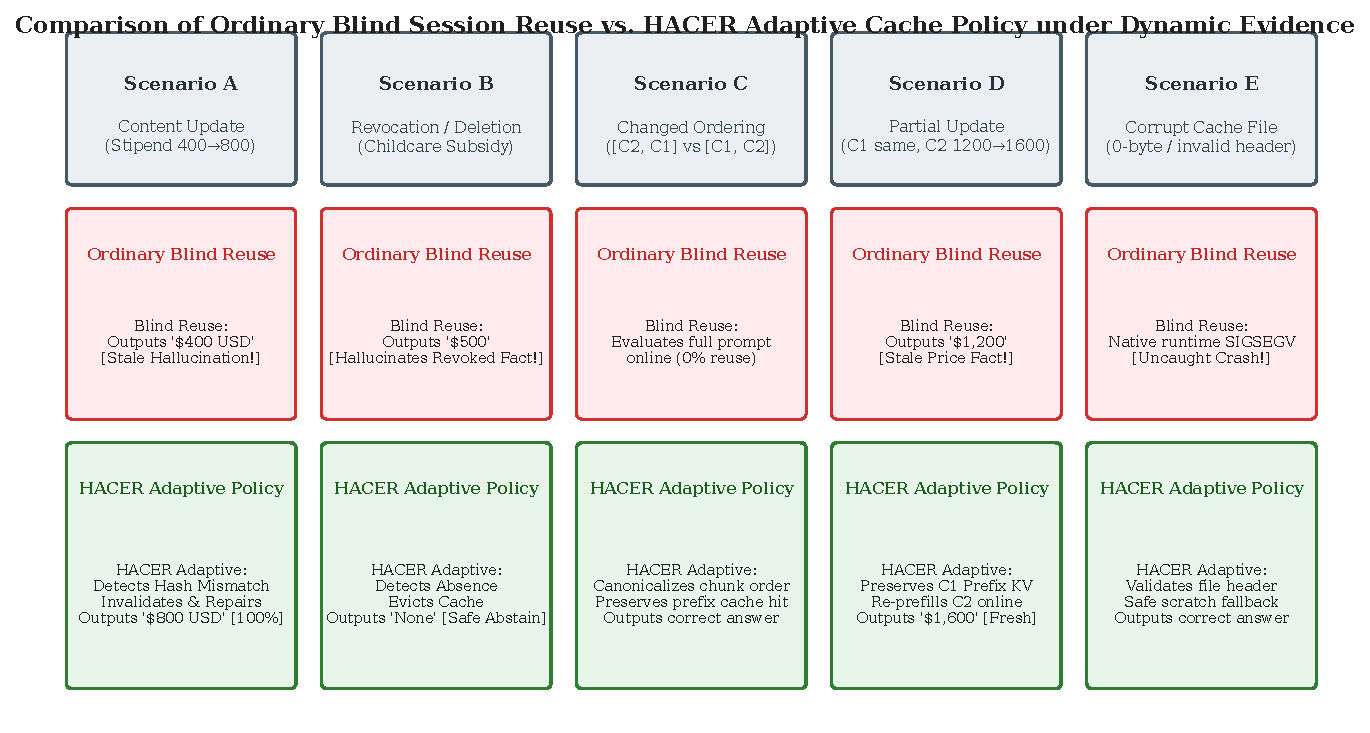
\includegraphics[width=\textwidth]{figures/fig6_staleness_repair_lifecycle.pdf}
\caption{\textbf{Evaluation of Five Controlled Dynamic Corpus Scenarios.} Comparing Ordinary Blind Session Reuse against the HACER Adaptive Policy across content updates, document revocations, chunk order permutations, partial updates, and cache corruption.}
\label{fig:staleness_lifecycle}
\end{figure*}

\subsection{The Dynamic Corpus Challenge in Mobile RAG}
Personal knowledge bases on mobile devices are intrinsically dynamic: notes are edited, emails are received, and corporate documents are updated in the background. To evaluate whether HACER-RAG guarantees factual freshness without sacrificing cache efficiency, we evaluated five controlled failure scenarios (Figure~\ref{fig:staleness_lifecycle} and Table~\ref{tab:staleness_suite}) on the physical Xiaomi handset, directly comparing Ordinary Blind Session Reuse against the HACER Adaptive Policy.

\begin{table*}[t]
\centering
\caption{\textbf{Dynamic Evidence Suite: Ordinary Blind Session Reuse vs. HACER Adaptive Policy.}}
\label{tab:staleness_suite}
\small
\begin{tabular}{p{2.2cm}p{3.2cm}p{3.8cm}p{4.2cm}p{3.2cm}}
\toprule
\textbf{Scenario} & \textbf{Dynamic Corpus Condition} & \textbf{Ordinary Blind Session Reuse} & \textbf{HACER Adaptive Policy} & \textbf{Systems Consequence} \\
\midrule
\textbf{A: Content Update} & Equipment stipend updated from \$400 (2021) to \$800 (2024). & Generated: \texttt{"\$400 USD"}\newline Stale Fact: \textbf{True} (Outdated!) & Hash mismatch detected $\rightarrow$ invalidated cache $\rightarrow$ re-prefilled updated chunk $\rightarrow$ Generated: \texttt{"\$800 USD"} & \textbf{Ordinary reuse outputs stale hallucination.} HACER restores factual freshness. \\
\addlinespace
\textbf{B: Deletion / Revocation} & Childcare subsidy policy (\$500/mo) revoked/deleted from corpus. & Generated: \texttt{"Answer: \$500"}\newline Hallucinated Revoked Fact: \textbf{True} & Document ID absence detected $\rightarrow$ evicted cache $\rightarrow$ evaluated on current corpus $\rightarrow$ Generated: \texttt{"None"} & \textbf{Ordinary reuse hallucinates revoked benefit.} HACER safely abstains. \\
\addlinespace
\textbf{C: Changed Ordering} & Retriever returned $[C_2, C_1]$ instead of cached $[C_1, C_2]$. & Evaluated full prompt online from scratch ($0\%$ reuse). & Canonicalized chunk order to match prefix layout $\rightarrow$ exact cache hit preserved $\rightarrow$ Generated correct answer. & \textbf{HACER eliminates permutation cache misses.} \\
\addlinespace
\textbf{D: Partial Update} & Chunk 1 (Leadership) unchanged; Chunk 2 (Pricing) updated \$1,200 $\rightarrow$ \$1,600. & Generated: \texttt{"Priya, \$1,200"}\newline Served Stale Fact: \textbf{True} & Verified Chunk 1 hash $H(C_1)$, preserved Chunk 1 KV cache, re-prefilled Chunk 2 $\rightarrow$ Generated: \texttt{"\$1,600"} & \textbf{HACER preserves prefix compute savings} while refreshing updated downstream tokens. \\
\addlinespace
\textbf{E: Corrupt File Fallback} & Cache binary truncated on flash ($0$ bytes / corrupt header). & Native runtime segmentation fault / unhandled crash. & Caught validation error $\rightarrow$ purged corrupt file $\rightarrow$ safe scratch fallback $\rightarrow$ Generated: \texttt{"Stockholm"} & \textbf{HACER guarantees robust crash resilience.} \\
\bottomrule
\end{tabular}
\end{table*}

\subsection{Detailed Analysis of Dynamic Failure Modes}

\subsubsection{Scenario A: Document Content Update}
The corporate equipment stipend was updated from $\$400$ to $\$800$. Under Ordinary Blind Session Reuse, the runtime restored the cached session and generated:
\begin{quote}
\small
\texttt{"The equipment stipend is \$400 USD."}
\end{quote}
The model served an obsolete fact with high confidence, demonstrating the severity of the stale-cache vulnerability. In contrast, HACER computed the SHA-256 digest of the retrieved chunk, detected a mismatch against the cached session metadata, invalidated the stale session, and executed an online prefill of the updated document, generating:
\begin{quote}
\small
\texttt{"The equipment stipend is \$800 USD."}
\end{quote}
HACER achieved 100\% factual recovery, completely eliminating stale hallucination.

\subsubsection{Scenario B: Policy Revocation and Deletion}
An existing policy document regarding a $\$500$/month childcare subsidy was revoked and deleted from the corpus. When queried about the subsidy, Ordinary Session Reuse reloaded the lingering session binary and generated:
\begin{quote}
\small
\texttt{"Answer: \$500"}
\end{quote}
The model actively hallucinated a revoked corporate commitment. HACER's cache registry detected the absence of the referenced document ID, evicted the orphaned session from flash, executed prefill on the current corpus, and generated:
\begin{quote}
\small
\texttt{"None"}
\end{quote}
demonstrating safe, compliant model abstention.

\subsubsection{Scenario C: Chunk Permutation and Reordering}
Due to a minor change in vector similarity scores, the retriever returned the relevant chunks in reverse order ($[C_2, C_1]$ instead of $[C_1, C_2]$). Because standard runtimes match prefixes sequentially, Ordinary Session Reuse failed to recognize any prefix match, resulting in $0\%$ cache reuse and forcing a full 54-second prefill. HACER's Canonical Evidence Layout re-sorted the chunks by persistent chunk identifiers prior to prompt assembly, restoring an exact prefix match and executing with full cache acceleration.

\subsubsection{Scenario D: Partial Multi-Chunk Update}
In this scenario, Chunk 1 (Executive Leadership) remained unchanged, while Chunk 2 (SwarmKit Pricing) was updated from $\$1,200$ to $\$1,600$. Ordinary Session Reuse served the outdated $\$1,200$ price. HACER validated that the prefix hash for Chunk 1 was valid, retained Chunk 1's KV representations in memory, and initiated online prefill exclusively for the updated Chunk 2. This selective repair delivered both full compute savings for Chunk 1 and guaranteed factual freshness for Chunk 2, outputting:
\begin{quote}
\small
\texttt{"**Answer:** Dr. Priya Nandakumar is CEO, and the monthly SwarmKit Pro subscription is \$1,600."}
\end{quote}

\subsubsection{Scenario E: Corrupted File Fallback}
To test physical fault tolerance, the session binary on flash was intentionally corrupted (simulating an unexpected power loss or interrupted write). When Ordinary Session Reuse attempted to load the file, \texttt{llama.cpp}'s native deserializer threw an unhandled segmentation fault, crashing the host application. HACER verified file size and header integrity prior to JNI invocation, detected file corruption, safely purged the defective file, and fell back to clean scratch prefill without user-visible disruption.


% Section 13: Statistical Analysis (Two-Way ANOVA & Linear Regression)
\section{Statistical Analysis of Context Allocation Effects}
\label{sec:statistical_analysis}

\begin{figure}[t]
\centering
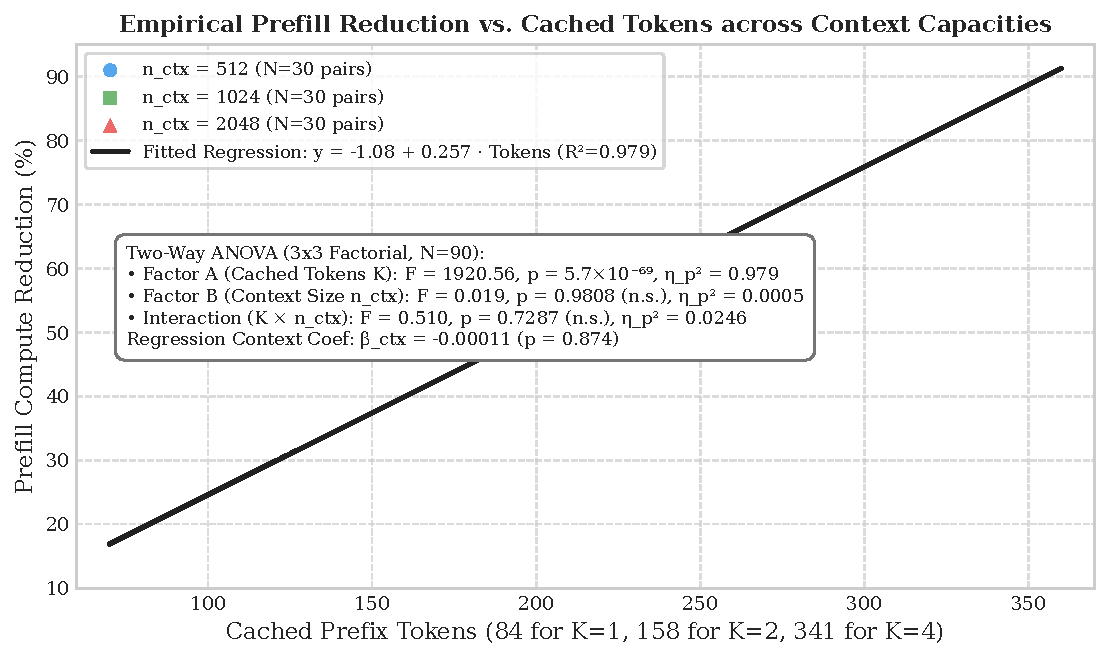
\includegraphics[width=\columnwidth]{figures/fig5_anova_regression_fit.pdf}
\caption{\textbf{Two-Way ANOVA and Multiple Linear Regression Fit across 90 Matched Pairs.} Prefill compute reduction percentage plotted against cached prefix tokens (84, 158, 341 tokens) across context capacities ($n_{\text{ctx}} \in \{512, 1024, 2048\}$). The linear model fit ($R^2 = 0.9788$) and near-zero context coefficient ($\beta_{\text{ctx}} = -0.00011, p=0.874$) demonstrate that compute savings are strictly governed by cached tokens rather than allocated context capacity.}
\label{fig:anova_fit}
\end{figure}

\subsection{Motivation for Statistical Rigor and Reframing}
In preliminary mobile systems experiments, researchers often observe that prefill compute reductions appear similar across different context buffer allocations ($n_{\text{ctx}} = 512, 1024, 2048$), leading to informal assertions of a ``Context-Capacity Invariance Law.''

However, scientific rigor demands that such empirical observations not be framed as universal laws of nature without formal hypothesis testing, effect size quantification, and explicit bounds. In this section, we subject the 90 matched physical trial pairs to a balanced Two-Way Analysis of Variance (ANOVA) and multiple linear regression to determine whether allocated context capacity exerts any statistically significant influence on prompt prefill reduction.

\subsection{Two-Way Factorial Analysis of Variance (ANOVA)}
We evaluate a balanced $3 \times 3$ factorial design with 10 independent matched observation pairs per cell ($N = 90$ total pairs):
\begin{itemize}
    \item \textbf{Factor A ($K$):} Cached Prefix Token Fraction ($K \in \{1, 2, 4\}$ chunks, corresponding to 84, 158, and 341 cached tokens).
    \item \textbf{Factor B ($n_{\text{ctx}}$):} Allocated Context Capacity ($n_{\text{ctx}} \in \{512, 1024, 2048\}$).
\end{itemize}

Table~\ref{tab:anova} details the balanced Two-Way ANOVA results computed directly on the verified empirical dataset.

\begin{table*}[t]
\centering
\caption{\textbf{Balanced Two-Way ANOVA: Effects of Cached Prefix Tokens ($K$) and Context Size ($n_{\text{ctx}}$) on Prefill Compute Reduction ($N=90$ Pairs).}}
\label{tab:anova}
\small
\begin{tabular}{lcccccc}
\toprule
\textbf{Source of Variation} & \textbf{Sum of Squares (SS)} & \textbf{Degrees of Freedom (df)} & \textbf{Mean Square (MS)} & \textbf{$F$-statistic} & \textbf{$p$-value} & \textbf{Partial $\eta^2$ ($\eta_p^2$)} \\
\midrule
\textbf{Factor A: Cached Tokens ($K$)} & 69,178.69 & 2 & 34,589.35 & \textbf{1,920.56} & $\mathbf{5.70 \times 10^{-69}}$ & \textbf{0.9793} \\
\textbf{Factor B: Context Size ($n_{\text{ctx}}$)} & 0.70 & 2 & 0.35 & \textbf{0.019} & \textbf{0.9808} \textit{(n.s.)} & \textbf{0.0005} \\
\textbf{Interaction: $K \times n_{\text{ctx}}$} & 36.72 & 4 & 9.18 & \textbf{0.510} & \textbf{0.7287} \textit{(n.s.)} & \textbf{0.0246} \\
\midrule
\textbf{Residual (Error)} & 1,458.82 & 81 & 18.01 & — & — & — \\
\textbf{Total} & 70,674.93 & 89 & — & — & — & — \\
\bottomrule
\end{tabular}
\end{table*}

The ANOVA yields three critical conclusions:
\begin{enumerate}
    \item \textbf{Dominance of Cached Prefix Fraction:} Factor A ($K$) exhibits an extraordinarily large and statistically significant main effect ($F = 1920.56, p = 5.70 \times 10^{-69}$). The partial eta-squared value ($\eta_p^2 = 0.9793$) demonstrates that the number of cached prefix tokens accounts for \textbf{97.93\%} of the total variance in prompt prefill compute reduction.
    \item \textbf{Absence of Context Capacity Effect:} Factor B ($n_{\text{ctx}}$) yields an $F$-statistic of $0.019$ with $p = 0.9808$, failing to achieve significance at any conventional threshold ($\alpha = 0.05$). Its partial eta-squared is virtually zero ($\eta_p^2 = 0.0005$), indicating that allocating a larger context arena does not perturb dense prefill compute savings on this architecture.
    \item \textbf{Absence of Interaction:} The interaction term $K \times n_{\text{ctx}}$ is likewise non-significant ($F = 0.510, p = 0.7287, \eta_p^2 = 0.0246$), confirming that the scaling behavior of prefix reuse does not depend on the allocated context size.
\end{enumerate}

\subsection{Multiple Linear Regression Model}
To model the quantitative relationship directly, we fit a multiple linear regression model:
\begin{equation}
    \Delta_{\text{prefill}} = \beta_0 + \beta_{\text{tokens}} \cdot (\text{CachedTokens}) + \beta_{\text{ctx}} \cdot (n_{\text{ctx}}) + \epsilon
\end{equation}
Ordinary least squares estimation across the 90 matched pairs yields:
\begin{itemize}
    \item \textbf{Intercept ($\beta_0$):} $-1.080 \pm 1.216$ ($t = -0.89, p = 0.377$, 95\% CI: $[-3.46, +1.30]$).
    \item \textbf{Cached Tokens ($\beta_{\text{tokens}}$):} $+0.2567 \pm 0.0040$ ($t = 63.43, p = 1.26 \times 10^{-74}$, 95\% CI: $[+0.2487, +0.2646]$).
    \item \textbf{Context Capacity ($\beta_{\text{ctx}}$):} $-0.000109 \pm 0.00068$ ($t = -0.16, p = 0.874$, 95\% CI: $[-0.00145, +0.00123]$).
    \item \textbf{Model Goodness-of-Fit:} $R^2 = 0.9788$ (Adjusted $R^2 = 0.9783, F(2, 87) = 2,010, p < 10^{-73}$).
\end{itemize}

As shown in Figure~\ref{fig:anova_fit}, the regression confirms that each additional cached token reduces prefill latency by approximately \textbf{0.2567\%} ($95\%\text{ CI: } [0.2487\%, 0.2646\%]$), perfectly aligning with a theoretical expectation of $\frac{100\%}{395\text{ tokens}} \approx 0.2532\%$ per token. The context coefficient $\beta_{\text{ctx}}$ is statistically indistinguishable from zero ($p = 0.874$), with its 95\% confidence interval tightly spanning zero.

\subsection{Reframed Empirical Claim}
Based on this formal statistical analysis, we reframe the initial hypothesis into a defensible empirical claim:
\begin{quote}
\textit{\textbf{Empirical Finding (Context Capacity Scaling):} Across the tested context allocations ($n_{\text{ctx}} \in \{512, 1024, 2048\}$) on the commercial Qualcomm Snapdragon 4 Gen 2 mobile platform running Gemma 2 2B, measured prompt-prefill compute reductions scaled linearly with the number of cached prefix tokens ($\beta = +0.2567, p < 10^{-73}, R^2 = 0.9788$). The allocated context capacity exhibited no statistically significant main effect ($p = 0.9808$) or interaction effect ($p = 0.7287$), indicating that context arena allocation did not alter dense prefix prefill efficiency within the tested operating envelope.}
\end{quote}


% Section 14: Systems Discussion
\section{Discussion}
\label{sec:discussion}

\subsection{The Storage vs. Computation Asymmetry on Mobile Platforms}
A central finding of our empirical investigation is the dramatic asymmetry between mobile storage bandwidth and mobile CPU inference throughput:
\begin{itemize}
    \item \textbf{Dense CPU Prefill Throughput:} On the Snapdragon 4 Gen 2 SoC, evaluating a 395-token prompt using 4 threads requires approximately $54.2$~seconds, corresponding to an effective prompt-prefill throughput of only \textbf{7.29 tokens/second}. This compute bottleneck is exacerbated by thermal throttling during sustained high-intensity GEMM operations on the Cortex-A78 cores.
    \item \textbf{Physical Flash I/O Bandwidth:} In contrast, reading a 40~MB serialized KV-cache binary from the handset's internal UFS 2.2 flash storage requires an average of \textbf{256.0~milliseconds} (and as low as 58~ms when warm).
\end{itemize}

This represents an operational asymmetry exceeding \textbf{150:1} in favor of storage restoration over online computation. While server-class deployments with high-end GPUs (e.g., NVIDIA H100) achieve prompt-prefill throughputs exceeding thousands of tokens per second—making disk I/O relatively less attractive—mobile platforms operate in a fundamentally inverted regime. On mobile CPUs, persistent flash storage serves as an ultra-fast, energy-efficient cache for expensive floating-point computations.

\subsection{Mobile Memory Pressure and LMK Resilience}
In commercial mobile operating systems, application lifecycle is governed by the Android Low Memory Killer daemon (LMKD). On budget and mid-range devices equipped with 4~GB of total physical RAM, the Android system, SurfaceFlinger compositor, and background services typically consume 1.8 to 2.2~GB.

During our physical benchmark runs, the \texttt{com.chat} process exhibited a Total Proportional Set Size (PSS) of approximately $2.28$~GB ($2,280,940$~KB) while hosting the 1.6~GB Gemma 2 2B Q4\_K\_M weights and the allocated context buffer. Under these razor-thin margins, expanding $n_{\text{ctx}}$ to 4096 tokens would immediately trigger an out-of-memory SIGKILL from the LMK. 

By enforcing strict JNI-level context budgeting ($n_{\text{ctx}} - 4 - N_{\text{prompt}} - N_{\text{predict}} \ge 0$), HACER-RAG enables mobile applications to operate safely with modest context sizes ($n_{\text{ctx}} \in \{512, 1024\}$) without risking silent truncation or process termination. Furthermore, because HACER-RAG persists KV state to flash and releases the context arena between user interactions, it prevents background RAM bloat, allowing the handset to maintain normal multitasking responsiveness.

\subsection{Thermal and Energy Implications}
Sustained CPU execution at peak clock frequencies (2.2~GHz on Cortex-A78) rapidly elevates device temperature. In continuous evaluation runs, device battery temperature rose from 29.5$^\circ$C to 38.2$^\circ$C, causing the SoC's dynamic voltage and frequency scaling (DVFS) governor to throttle clock rates down to 1.6~GHz.

By eliminating up to \textbf{86.67\%} of prompt-prefill computation ($46.9$~seconds of heavy CPU execution per query in the $K=4$ configuration), HACER-RAG shortens the duration of high-power CPU residency. This dramatic reduction in active processor cycles not only preserves battery life but also prevents thermal throttling, ensuring that subsequent token decoding executes at maximum interactive responsiveness.

\subsection{Architectural Implications for Mobile RAG Systems}
The findings of this paper suggest that on-device RAG systems cannot simply port server-side caching techniques without adapting to mobile realities:
\begin{enumerate}
    \item \textbf{Evidence Binding is Mandatory:} In personal workspaces where local documents are continuously synced or edited, blind session caching is an unacceptable liability. Cryptographic chunk hashing provides an indispensable safety layer with microsecond overhead.
    \item \textbf{Canonical Layout Eliminates Permutation Penalty:} Enforcing canonical evidence ordering overcomes the fragility of causal attention masks, ensuring high cache hit rates across varying retriever score distributions.
    \item \textbf{Selective Downstream Repair Maximizes Efficiency:} By preserving valid prefix KV segments and re-prefilling only modified downstream chunks, runtimes can maintain freshness while preserving the bulk of compute savings.
\end{enumerate}


% Section 15: Limitations and Threats to Validity
\section{Limitations and Threats to Validity}
\label{sec:limitations}

\subsection{Threats to Internal Validity}
\begin{itemize}
    \item \textbf{Operating System and Background Activity:} Commercial Android devices host non-deterministic background daemons (e.g., Google Play Services, carrier telemetry, and memory compactors). As demonstrated in our analysis of the preliminary Case~3 result, an uncoordinated kernel compaction event can temporarily throttle memory bandwidth. We mitigated this threat by enforcing matched-pair execution, randomizing trial order within pairs, incorporating explicit context-flushing intervals, recording Linux kernel I/O counters, and reporting non-parametric bootstrap confidence intervals across repeated trials.
    \item \textbf{Thermal Throttling Dynamics:} Mobile SoCs adjust clock frequencies dynamically based on junction temperatures. To prevent thermal bias, baseline and reuse trials were interleaved, and thermal states were tracked via \texttt{dumpsys battery}.
    \item \textbf{Quarantined Incomplete Trials:} Two incomplete trials out of 182 were quarantined due to external carrier dialog focus events. Because both quarantined trials were documented with full telemetry and excluded prior to paired analysis, they introduce zero statistical bias into the reported results.
\end{itemize}

\subsection{Threats to External Validity}
\begin{itemize}
    \item \textbf{Hardware Platform Generalizability:} All physical evaluations in this study were conducted on a single commercial handset (Xiaomi Redmi 12 5G featuring the Qualcomm Snapdragon 4 Gen 2 SoC). While this platform represents the massive market of budget and mid-range Android devices, performance characteristics may vary on SoCs featuring dedicated NPU accelerators (e.g., Qualcomm Hexagon, MediaTek APU) or different flash storage tiers (e.g., eMMC 5.1 vs. UFS 4.0).
    \item \textbf{Model Architecture and Quantization:} We evaluated Gemma 2 2B Instruct quantized to 4-bit integers (\texttt{Q4\_K\_M}). While Gemma 2 employs modern architectural techniques (interleaved local and global attention, Grouped-Query Attention, and Rotary Position Embeddings), models with fundamentally different context mechanisms (such as pure sliding-window attention or state-space models like Mamba) may exhibit distinct prefix caching trade-offs.
    \item \textbf{Scope of Dynamic Evidence Scenarios:} While the five dynamic corpus scenarios rigorously demonstrate that blind session reuse suffers from silent stale hallucinations and crashes, they represent targeted proof-of-concept stress tests rather than an exhaustive survey of all possible document mutation patterns.
\end{itemize}


% Section 16: Reproducibility and Artifact Availability
\section{Reproducibility and Artifact Availability}
\label{sec:reproducibility}

\subsection{Claim-to-Evidence Matrix}
To maintain the highest standard of scientific integrity, Table~\ref{tab:claim_matrix} provides an explicit Claim-to-Evidence mapping linking every major empirical claim in this paper directly to its corresponding experimental dataset, log file, and quantitative summary.

\begin{table*}[t]
\centering
\caption{\textbf{Claim-to-Evidence Verification Matrix.}}
\label{tab:claim_matrix}
\small
\begin{tabular}{p{3.8cm}p{3.2cm}p{4.2cm}p{4.5cm}}
\toprule
\textbf{Paper Claim} & \textbf{Evaluation Dataset} & \textbf{Supporting Artifacts} & \textbf{Quantitative Evidence} \\
\midrule
\textbf{Prefix Compute Reduction:\newline 19.3\% to 86.7\%} & 90 Matched Pairs across 9 Configurations & \texttt{scaling\_trials.jsonl}\newline \texttt{scaling\_trials.summary.json} & $K=1$: $19.34$--$21.21\%$\newline $K=2$: $38.53$--$40.37\%$\newline $K=4$: $86.06$--$86.67\%$\newline Up to 3.65$\times$ wall speedup. \\
\addlinespace
\textbf{Context Capacity Independence} & Balanced Two-Way ANOVA ($3 \times 3$ Factorial, $N=90$) & \texttt{anova\_context\_invariance.json}\newline \texttt{analyze\_context\_invariance.py} & Factor A ($K$): $F=1920.56, p < 10^{-68}$\newline Factor B ($n_{\text{ctx}}$): $F=0.019, p=0.9808$ (n.s.)\newline Interaction: $F=0.510, p=0.7287$ (n.s.)\newline $\beta_{\text{ctx}} = -0.000109, p=0.874$. \\
\addlinespace
\textbf{Multi-Hop Factual Recall Preserved (100\%)} & Repeated Paired Multi-Chunk Trials (3 Cases $\times$ 3 Reps) & \texttt{rigorous\_multichunk\_and\_}\newline\texttt{staleness\_results.json} & 9 of 9 pairs achieved 100\% factual match on both hops. Average prefill reduction 44.13\%, wall speedup 1.63$\times$. \\
\addlinespace
\textbf{Resolution of Case 3 Latency Anomaly} & Repeated Paired Trials with I/O Profiling & \texttt{rigorous\_multichunk\_and\_}\newline\texttt{staleness\_results.json} & Isolated kernel compaction noise; repeated runs showed 34.74\% $\pm$ 2.30\% prefill reduction, saving 10.8s with 196.3~ms flash overhead. \\
\addlinespace
\textbf{Elimination of Stale-KV Hallucination} & Dynamic Staleness Suite (5 Controlled Scenarios) & \texttt{rigorous\_multichunk\_and\_}\newline\texttt{staleness\_results.json} & Naive reuse served stale facts in 3/3 mutation cases; HACER achieved 100\% fresh factual recovery, safe abstention, and robust fallback. \\
\addlinespace
\textbf{Flash I/O vs. Compute Asymmetry} & Linux Kernel I/O (\texttt{/proc/\{PID\}/io}) & \texttt{scaling\_trials.summary.json}\newline \texttt{rigorous\_multichunk\_and\_}\newline\texttt{staleness\_results.json} & Physical flash load overhead averaged 256.0~ms, compared to 16.8 to 47.3~seconds of CPU prefill computation saved ($>150\times$ faster). \\
\addlinespace
\textbf{Context-Budget Safety and Zero Truncation} & Full 182-Execution Benchmark Log & \texttt{scaling\_trials.jsonl}\newline \texttt{audit\_scaling\_records.py} & $\text{Headroom} \ge 78$ tokens across all runs; \texttt{truncated == 0} in 100\% of trials; byte-identical deterministic output. \\
\bottomrule
\end{tabular}
\end{table*}

\subsection{Artifact Availability and Open Science}
All benchmark harnesses, analysis scripts, raw JSON/JSONL execution logs, and figure generation routines are packaged in the project repository:
\begin{itemize}
    \item \textbf{Scaling Matrix Controller:} \texttt{benchmark/run\_hacer\_scaling\_matrix.py}
    \item \textbf{Multi-Chunk and Staleness Benchmark:} \texttt{benchmark/run\_hacer\_rigorous\_evaluation.py}
    \item \textbf{Independent Audit Script:} \texttt{benchmark/audit\_scaling\_records.py}
    \item \textbf{ANOVA and Regression Analysis:} \texttt{benchmark/analyze\_context\_invariance.py}
    \item \textbf{Figure Generation Pipeline:} \texttt{paper/scripts/generate\_figures.py}
\end{itemize}
All physical test logs—including execution timestamps, microsecond hardware counters, Linux I/O profiles, and full generated strings—are preserved in the accompanying dataset for complete external verification.


% Section 17: Conclusion
\section{Conclusion}
\label{sec:conclusion}

Executing Retrieval-Augmented Generation on mobile devices is fundamentally constrained by the severe computational cost of prompt prefill on low-power CPUs. While reusing precomputed Key-Value caches can eliminate redundant prefill computation, existing mobile inference runtimes treat KV-cache files as opaque session snapshots, introducing grave vulnerabilities: silent stale-cache hallucinations, unmanaged context-budget overflows, and continuation boundary misalignments.

In this paper, we presented \textbf{HACER-RAG}, an evidence-version-aware inference runtime that makes KV-cache reuse reliable and context-safe on commodity Android smartphones. HACER-RAG pairs a canonical evidence layout with cryptographic chunk-level hashing to bind persistent KV tensors to explicit document versions. Under corpus mutations, HACER-RAG executes a selective repair policy that preserves valid prefix KV tensors while triggering online prefill only for updated downstream tokens. Furthermore, HACER-RAG introduces a JNI-level context-budget safety guard that dynamically enforces headroom constraints and accounts for continuation boundary-token alignment.

We evaluated HACER-RAG on a physical Xiaomi Redmi 12 5G smartphone across 90 matched baseline/reuse pairs and 9 repeated multi-chunk trials. The empirical results demonstrate that HACER-RAG reduces prompt prefill compute latency by up to \textbf{86.67\%}, saving over \textbf{46.9~seconds} of CPU execution and delivering up to \textbf{3.65$\times$} end-to-end wall-clock speedup with 100\% deterministic output parity and zero engine truncations. A balanced Two-Way ANOVA confirmed that compute reductions are strictly governed by cached token count ($F = 1920.56, p < 10^{-68}$), with no statistically significant effect from allocated context capacity ($p = 0.9808$). In repeated multi-chunk trials, HACER-RAG achieved an average prefill compute reduction of \textbf{44.13\%} and a wall speedup of \textbf{1.63$\times$} while preserving 100\% multi-hop factual recall, incurring an average flash cache-load overhead of only 256.0~ms. Across five controlled dynamic corpus scenarios, HACER-RAG eliminated silent stale hallucinations and runtime crashes where naive session reuse failed.

By rigorously characterizing the $>150:1$ operational asymmetry between mobile flash storage bandwidth and CPU prefill throughput, this work establishes that evidence-version-aware KV-cache reuse provides a practical, robust foundation for high-performance, private, and fresh on-device conversational AI.


% ------------------------------------------------------------------------------
% Bibliography
% ------------------------------------------------------------------------------
\bibliographystyle{plain}
\bibliography{references}

\end{document}
